\section{Índices de governo eletrônico}

Existem 4 tipos de índices de governo eletrônico, segundo \cite{martinez2022egovernment}: EDGI da ONU, GTMI do Banco Mundial, DESI da Comissão Europeia da União Europeia e DGI da OECD.

A não escolha do DESI foi motivada pela explicação de \cite{desi_2022} de como ó índice funciona. De acordo com \cite{desi_2022}, como o DESI é administrado pela Comissão Europeia da UE, ele foca no análise individual de cada Estado membro da UE para que eles possam identificar áreas que precisam de ações prioritárias. Além disso, os relatórios do DESI possuem capítulos temáticos que providenciam analises a nível supranacional em áreas de áreas chave de política digital.

\subsection{EGDI}

O EGDI apresenta o estado de desenvolvimento de governo eletrônico dos Estados membro da ONU. O índice incorpora as características de acesso, tais como níveis de infraestrutura e educacional para mostrar como um país está usando as tecnologias de informação para promover acesso e inclusão do seu povo \cite{ONU_egdi}.

\cite{ONU_egdi} afirma que o EGDI é uma mensuração composta formada por 3 importantes dimensões do governo eletrônico: provisão de serviços online, conectividade de telecomunicação e capacidade humana.

Os componentes do EGDI são:

\begin{figure}[H]
	\centering
	\caption{Componentes do EGDI}
	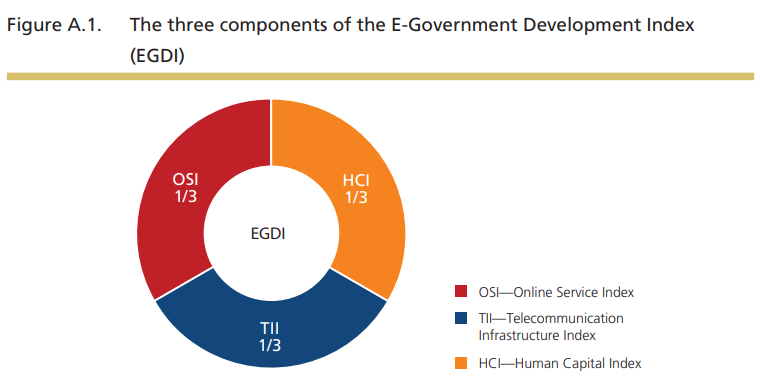
\includegraphics[width=1\linewidth]{figuras/egdi/egdi_componentes.png}
	\label{fig:egdi_componentes}
	\footnotesize{Fonte: \cite{ONU_egdi_methodology}}
\end{figure}


Adicionalmente, cada componente citado na figura \ref{fig:egdi_componentes} será descrito individualmente nas subseções \ref{epart}, \ref{osi}, \ref{hci} e \ref{tii}.

A figura \ref{fig:boxplot_egov_global} contém um diagrama de caixa que representa o EGDI global.

\begin{figure}[H]
	\centering
	\caption{E-Government Development Index}
	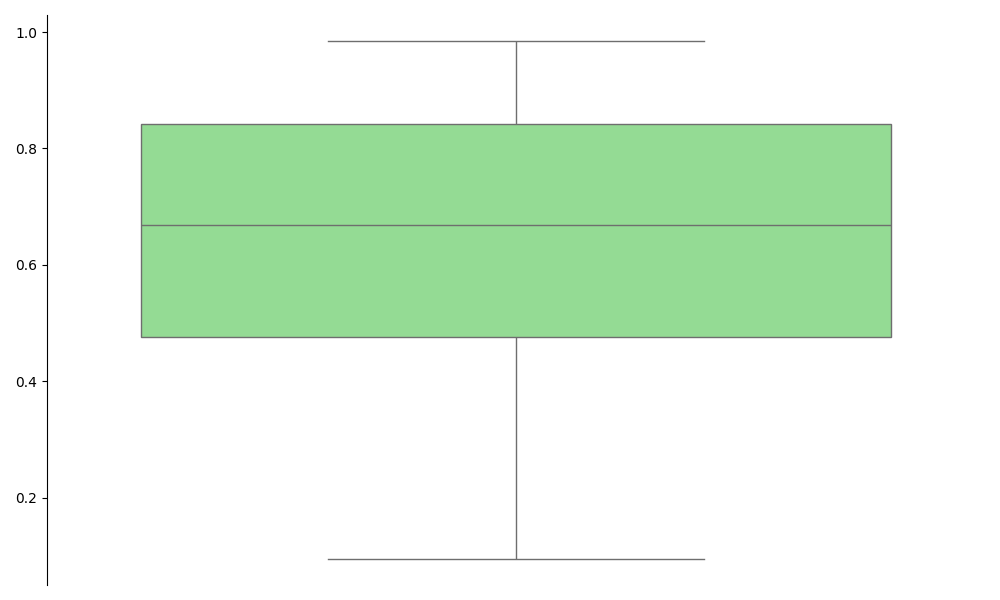
\includegraphics[width=1\linewidth]{figuras/egdi/boxplot_egov_global.png}
	\label{fig:boxplot_egov_global}
	\footnotesize{Fonte: baseado em \cite{ONU_edgi_mapa}.}
\end{figure}

A figura \ref{fig:boxplot_egov_global} revela uma ampla distribuição de valores, variando de aproximadamente 0,08 a 1,0. A mediana, em torno de 0,67, indica que metade dos países tem um desempenho igual ou inferior a esse valor. Os 50\% centrais dos dados (o intervalo interquartil) estão concentrados entre 0,47 e 0,84. A ausência de pontos atípicos sugere que a variação do índice entre os países é contínua e sem desvios extremos.

\subsubsection{E-Participation Index}
\label{epart}

\cite{ONU_egdi} argumenta que o \textbf{E-Participation Index} deriva do EGDI como índice suplementar ao relatório \textbf{E-Government Survey}. Os componentes do índice são: \textbf{E-information}, \textbf{E-consultation} e \textbf{E-decision-making}. 

\textbf{E-information} fala sobre a facilitação da participação dos cidadãos via informações públicas e acesso a informação sem necessidade de pedido ou sob demanda. \textbf{E-consultation} diz respeito ao engajamento dos cidadãos em contribuições e deliberações sobre políticas publicas e serviços públicos. \textbf{E-decision-making} engloba o empoderamento dos cidadãos via a opção de coparticipação na elaboração de políticas e coprodução de componentes de serviços e entrega de modalidades.

\cite{ONU_egdi} esclarece que o \textbf{E-Participation Index} de um país reflete os mecanismos do índice que são empregados pelo governo quando se faz comparações com todos outros países. 

O propósito dessa medição não é prescrever qualquer prática especificam, no entanto oferece perspectivas de como países diferentes estão usando ferramentas online para promover interação entre o governo e seu povo, bem como, entre as pessoas para benefícios de todos.

A figura \ref{fig:boxplot_epart_global} contém um diagrama de caixa que representa o \textbf{E-Participation Index} global.

\begin{figure}[H]
	\centering
	\caption{E-Participation Index global}
	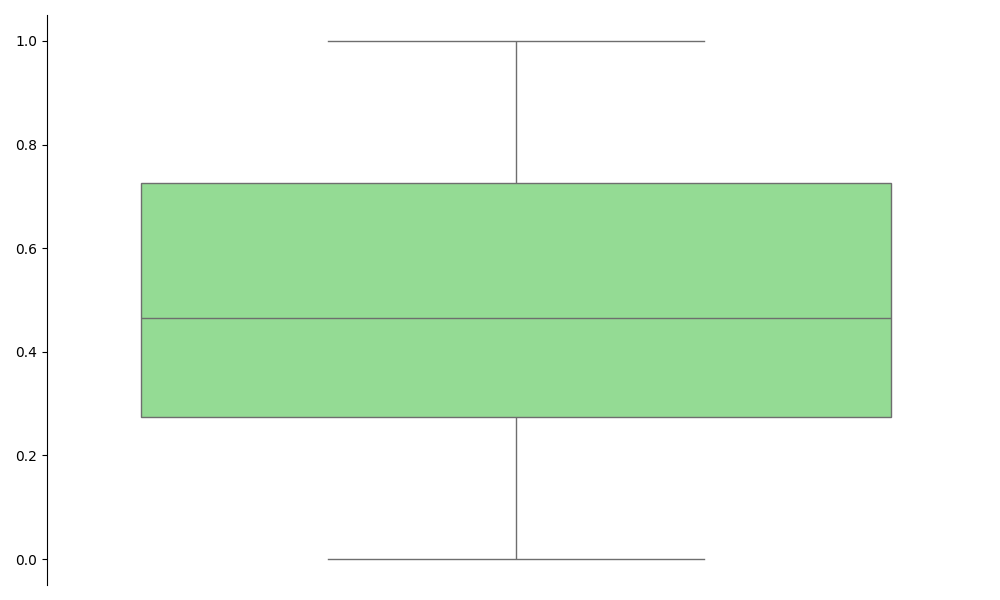
\includegraphics[width=1\linewidth]{figuras/egdi/boxplot_epart_global.png}
	\label{fig:boxplot_epart_global}
	\footnotesize{Fonte: baseado em \cite{ONU_edgi_mapa}.}
\end{figure}

A figura \ref{fig:boxplot_epart_global} ilustra a distribuição do Índice de Serviço Online. O gráfico mostra que a mediana do índice global está próxima de 0,58. Os 50\% centrais dos dados, representados pela caixa, estão no intervalo entre 0,36 e 0,80. Os bigodes do gráfico indicam uma variação de aproximadamente 0,0 a 1,0, abrangendo todo o espectro de valores possíveis. Em resumo, o índice apresenta uma ampla dispersão, mas com a maioria dos países concentrada na faixa intermediária a alta, e a mediana ligeiramente acima do ponto central da escala.

\subsubsection{Online Service Index}
\label{osi}

\begin{figure}[H]
	\centering
	\caption{Online Service Index global}
	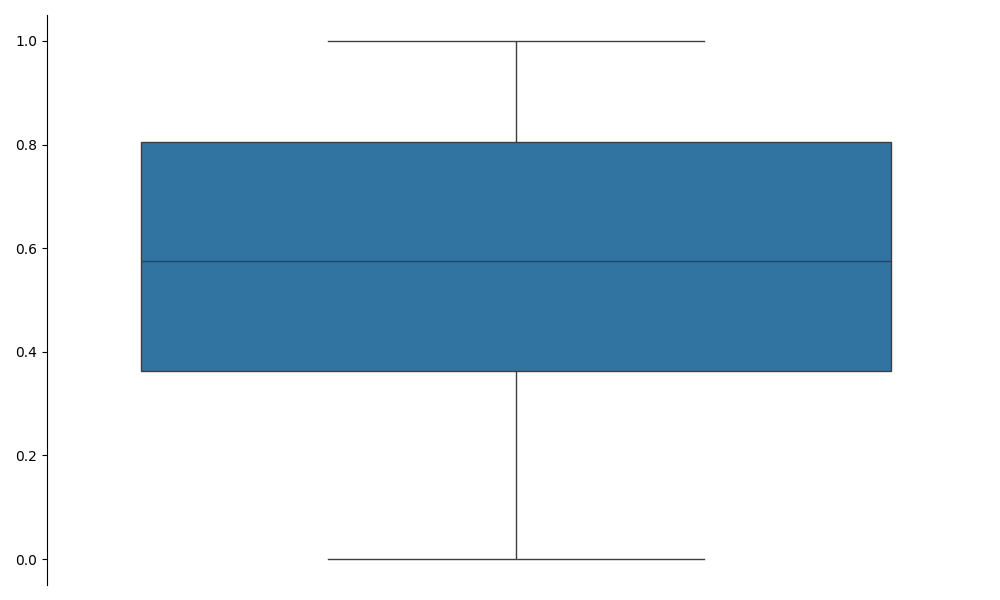
\includegraphics[width=1\linewidth]{figuras/egdi/boxplot_osi_global.png}
	\label{fig:boxplot_osi_global}
	\footnotesize{Fonte: baseado em \cite{ONU_edgi_mapa}.}
\end{figure}

\subsubsection{Human Capital Index}
\label{hci}

\begin{figure}[H]
	\centering
	\caption{Human Capital Index global}
	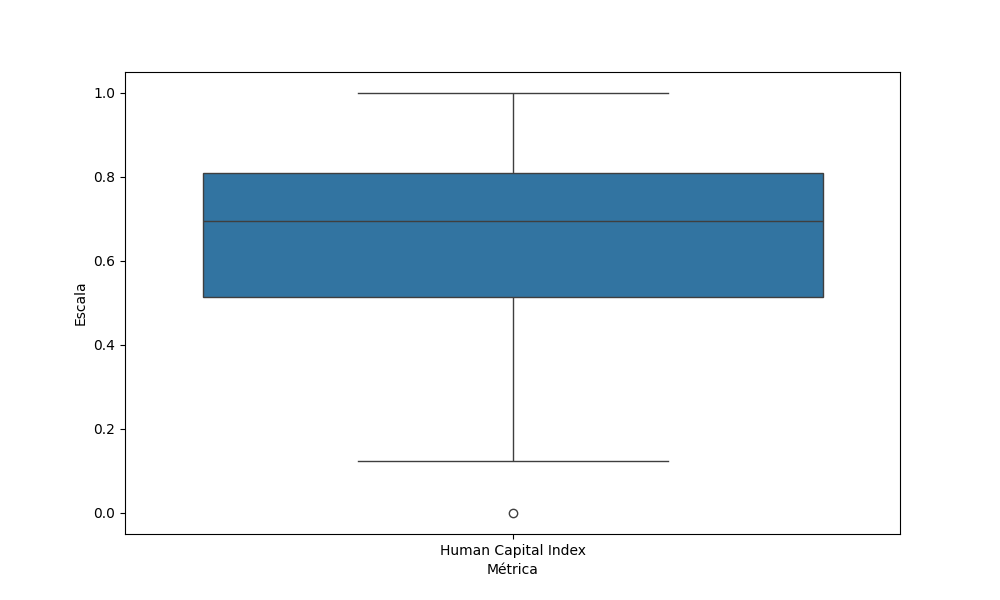
\includegraphics[width=1\linewidth]{figuras/egdi/boxplot_hci_global.png}
	\label{fig:boxplot_hci_global}
	\footnotesize{Fonte: baseado em \cite{ONU_edgi_mapa}.}
\end{figure}

\subsubsection{Telecommunication Infrastructure Index}
\label{tii}

\begin{figure}[H]
	\centering
	\caption{Telecommunication Infrastructure Index global}
	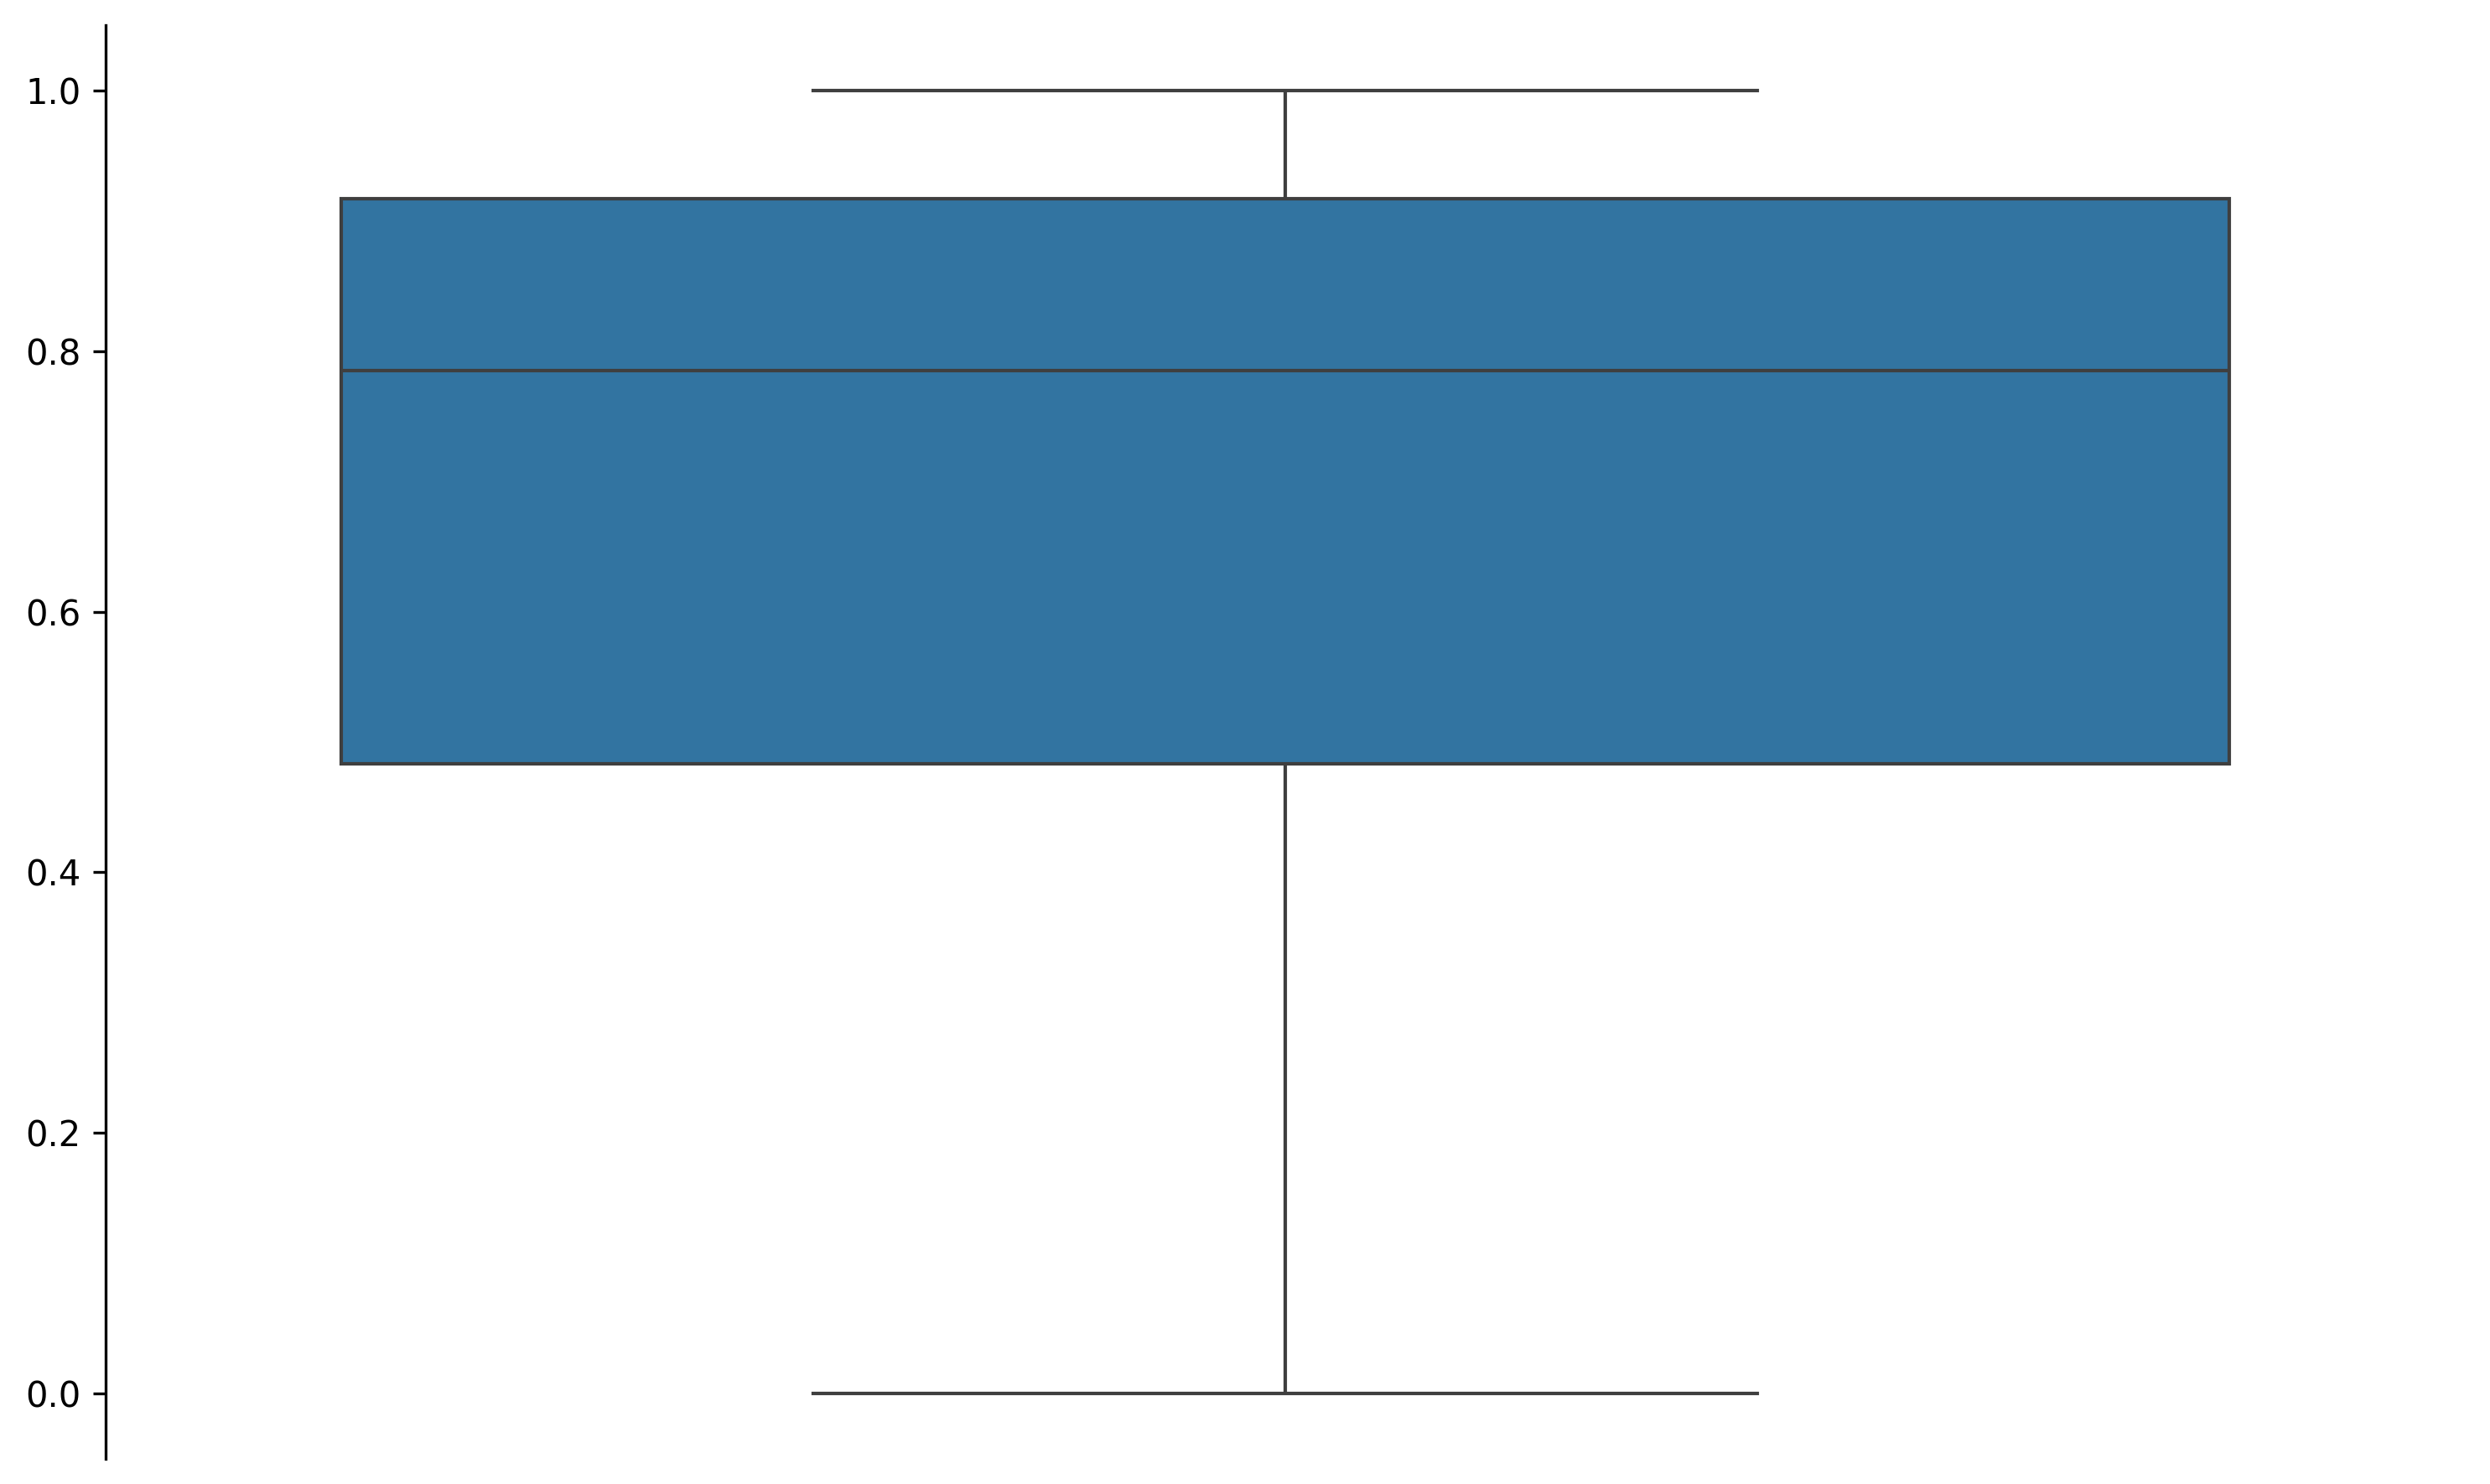
\includegraphics[width=1\linewidth]{figuras/egdi/boxplot_tci_global.png}
	\label{fig:boxplot_tci_global}
	\footnotesize{Fonte: baseado em \cite{ONU_edgi_mapa}.}
\end{figure}

\subsubsection{EGDI do Brasil}

\begin{figure}[H]
	\centering
	\caption{Evolução do EGDI do Brasil}
	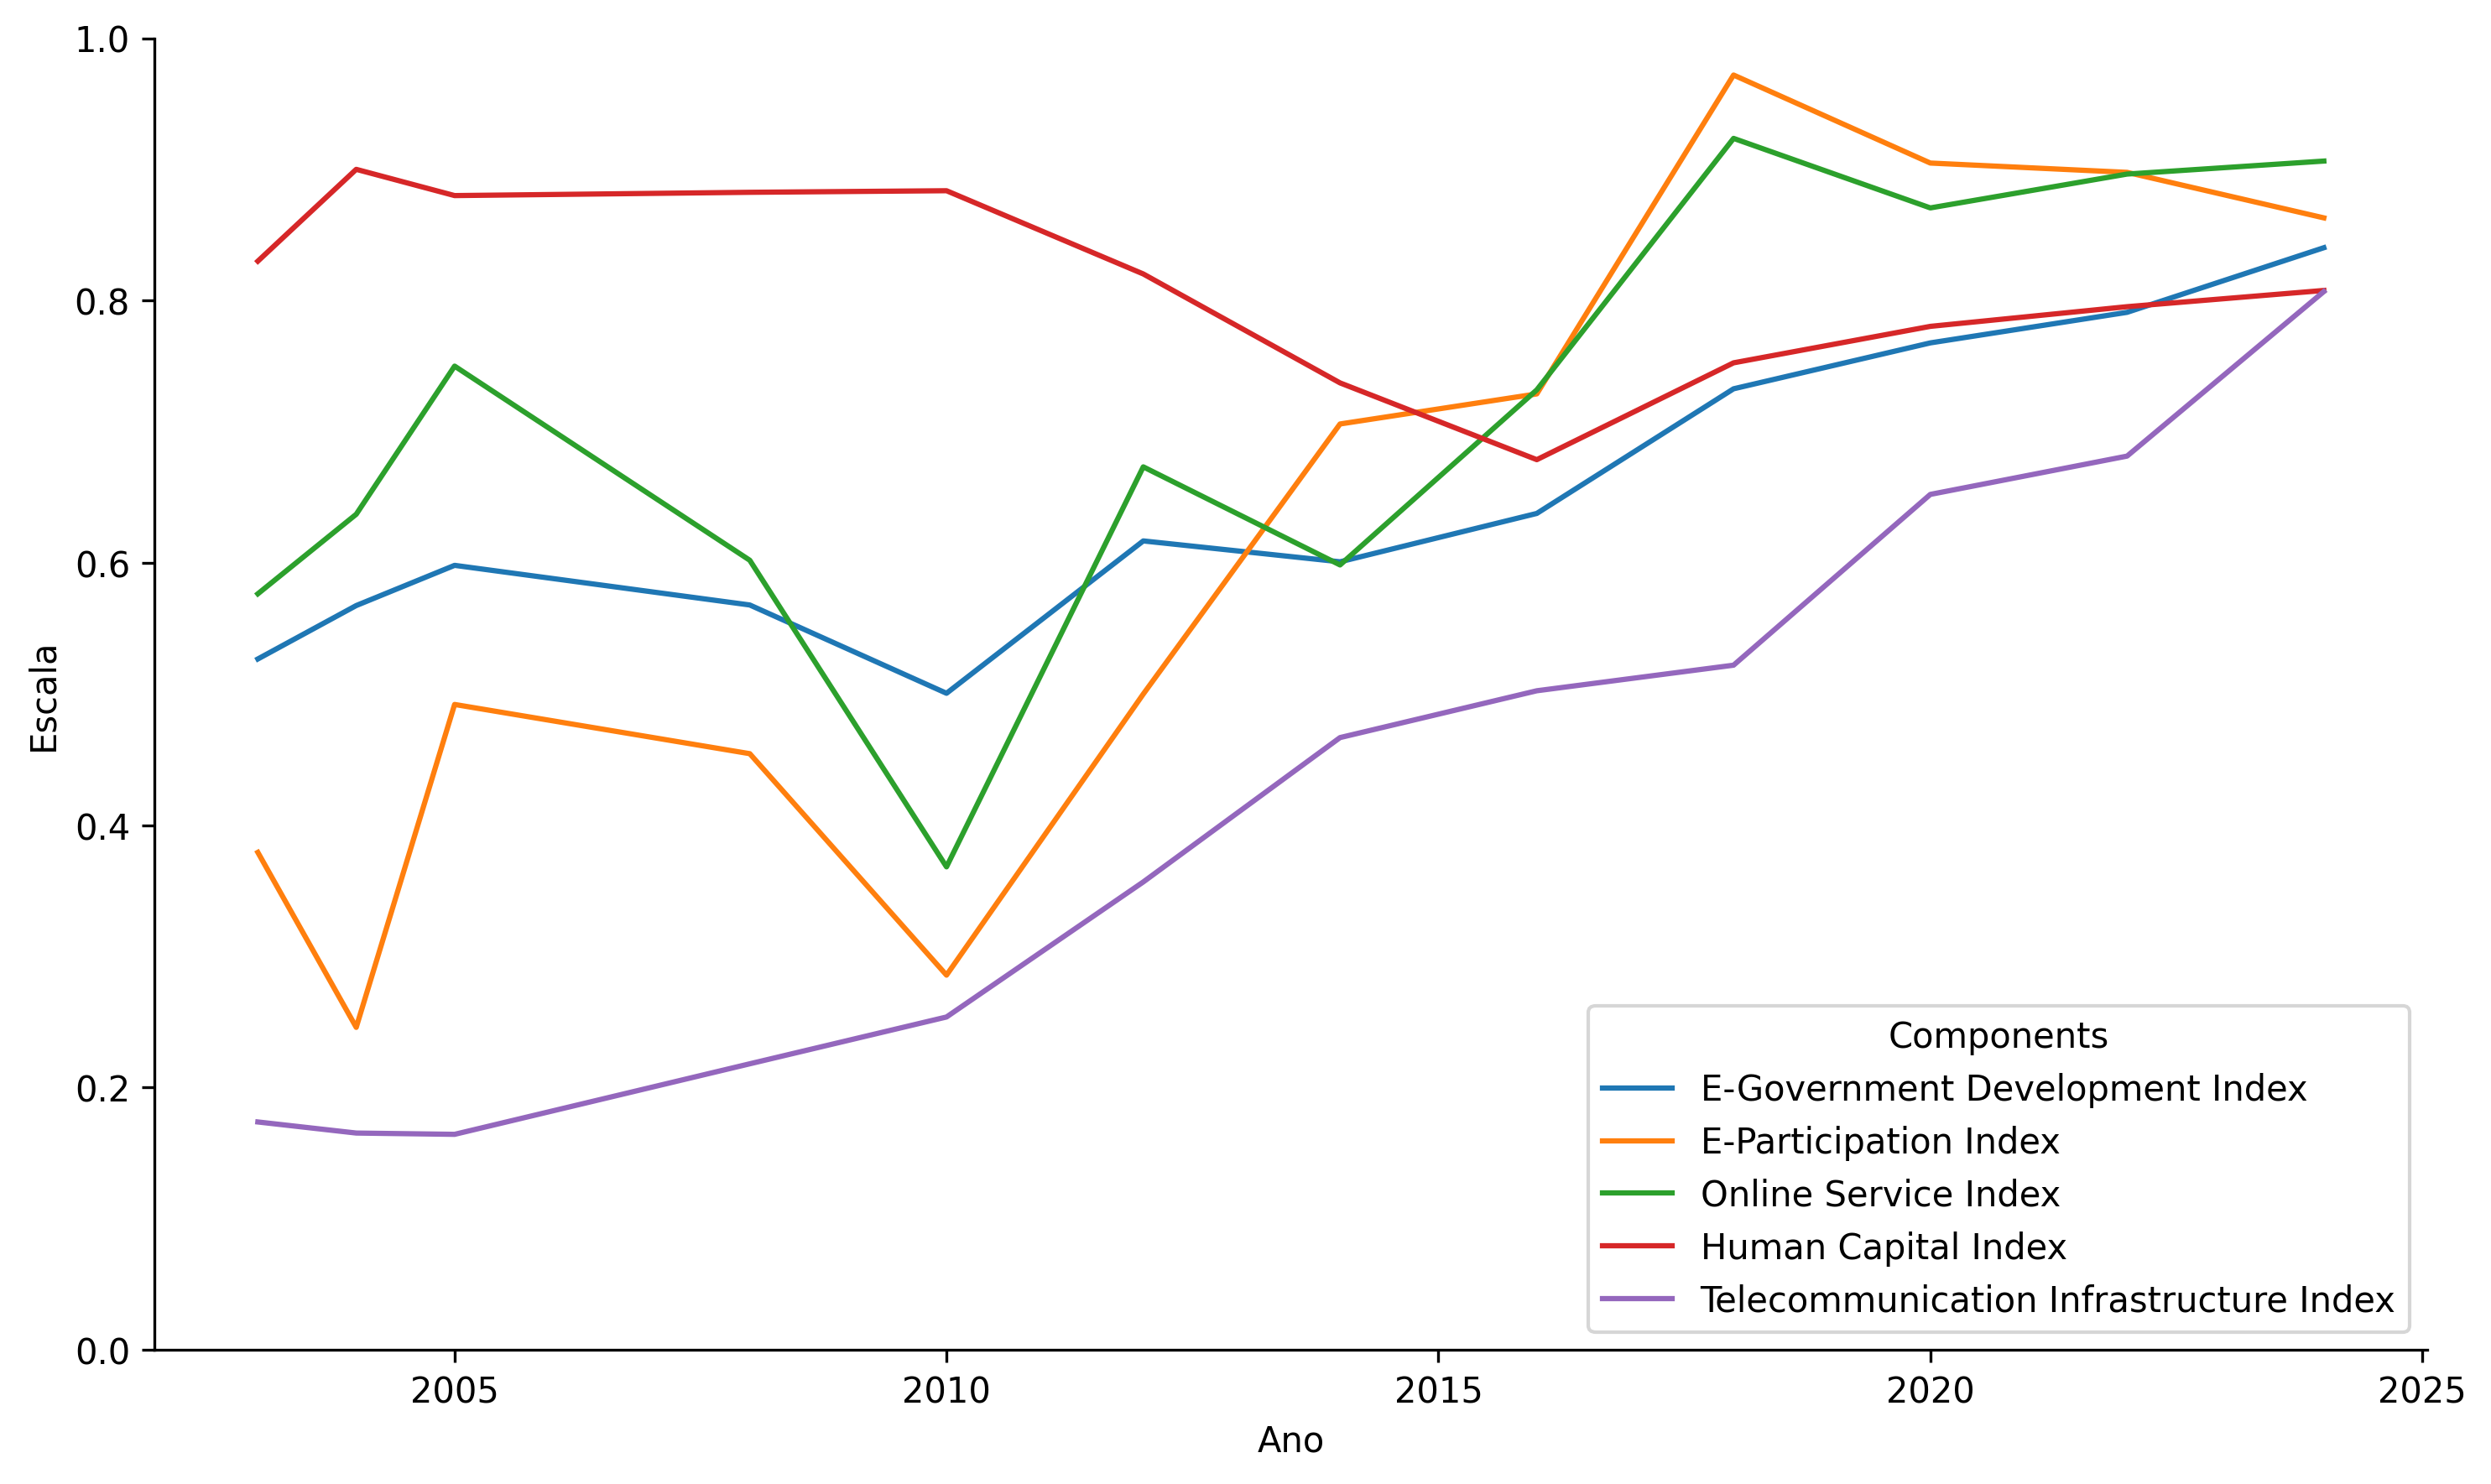
\includegraphics[width=1\linewidth]{figuras/egdi/lineplot_egdi_brasil.png}
	\label{fig:lineplot_egdi_brasil}
	\footnotesize{Fonte: baseado em \cite{ONU_edgi_mapa}.}
\end{figure}

\paragraph{E-Government Index}

\begin{figure}[H]
	\centering
	\caption{EGDI do Brasil: E-Government Index}
	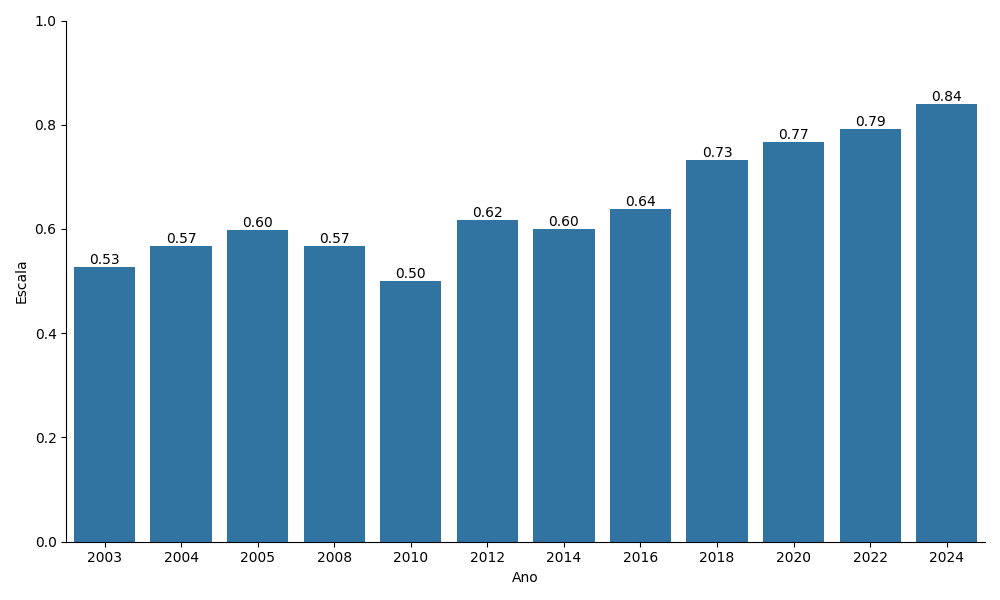
\includegraphics[width=1\linewidth]{figuras/egdi/egdi_brasil_egov.png}
	\label{fig:egdi_brasil_egov}
	\footnotesize{Fonte: baseado em \cite{ONU_edgi_mapa}.}
\end{figure}

\paragraph{E-Participation Index}

\begin{figure}[H]
	\centering
	\caption{EGDI do Brasil: E-Participation Index}
	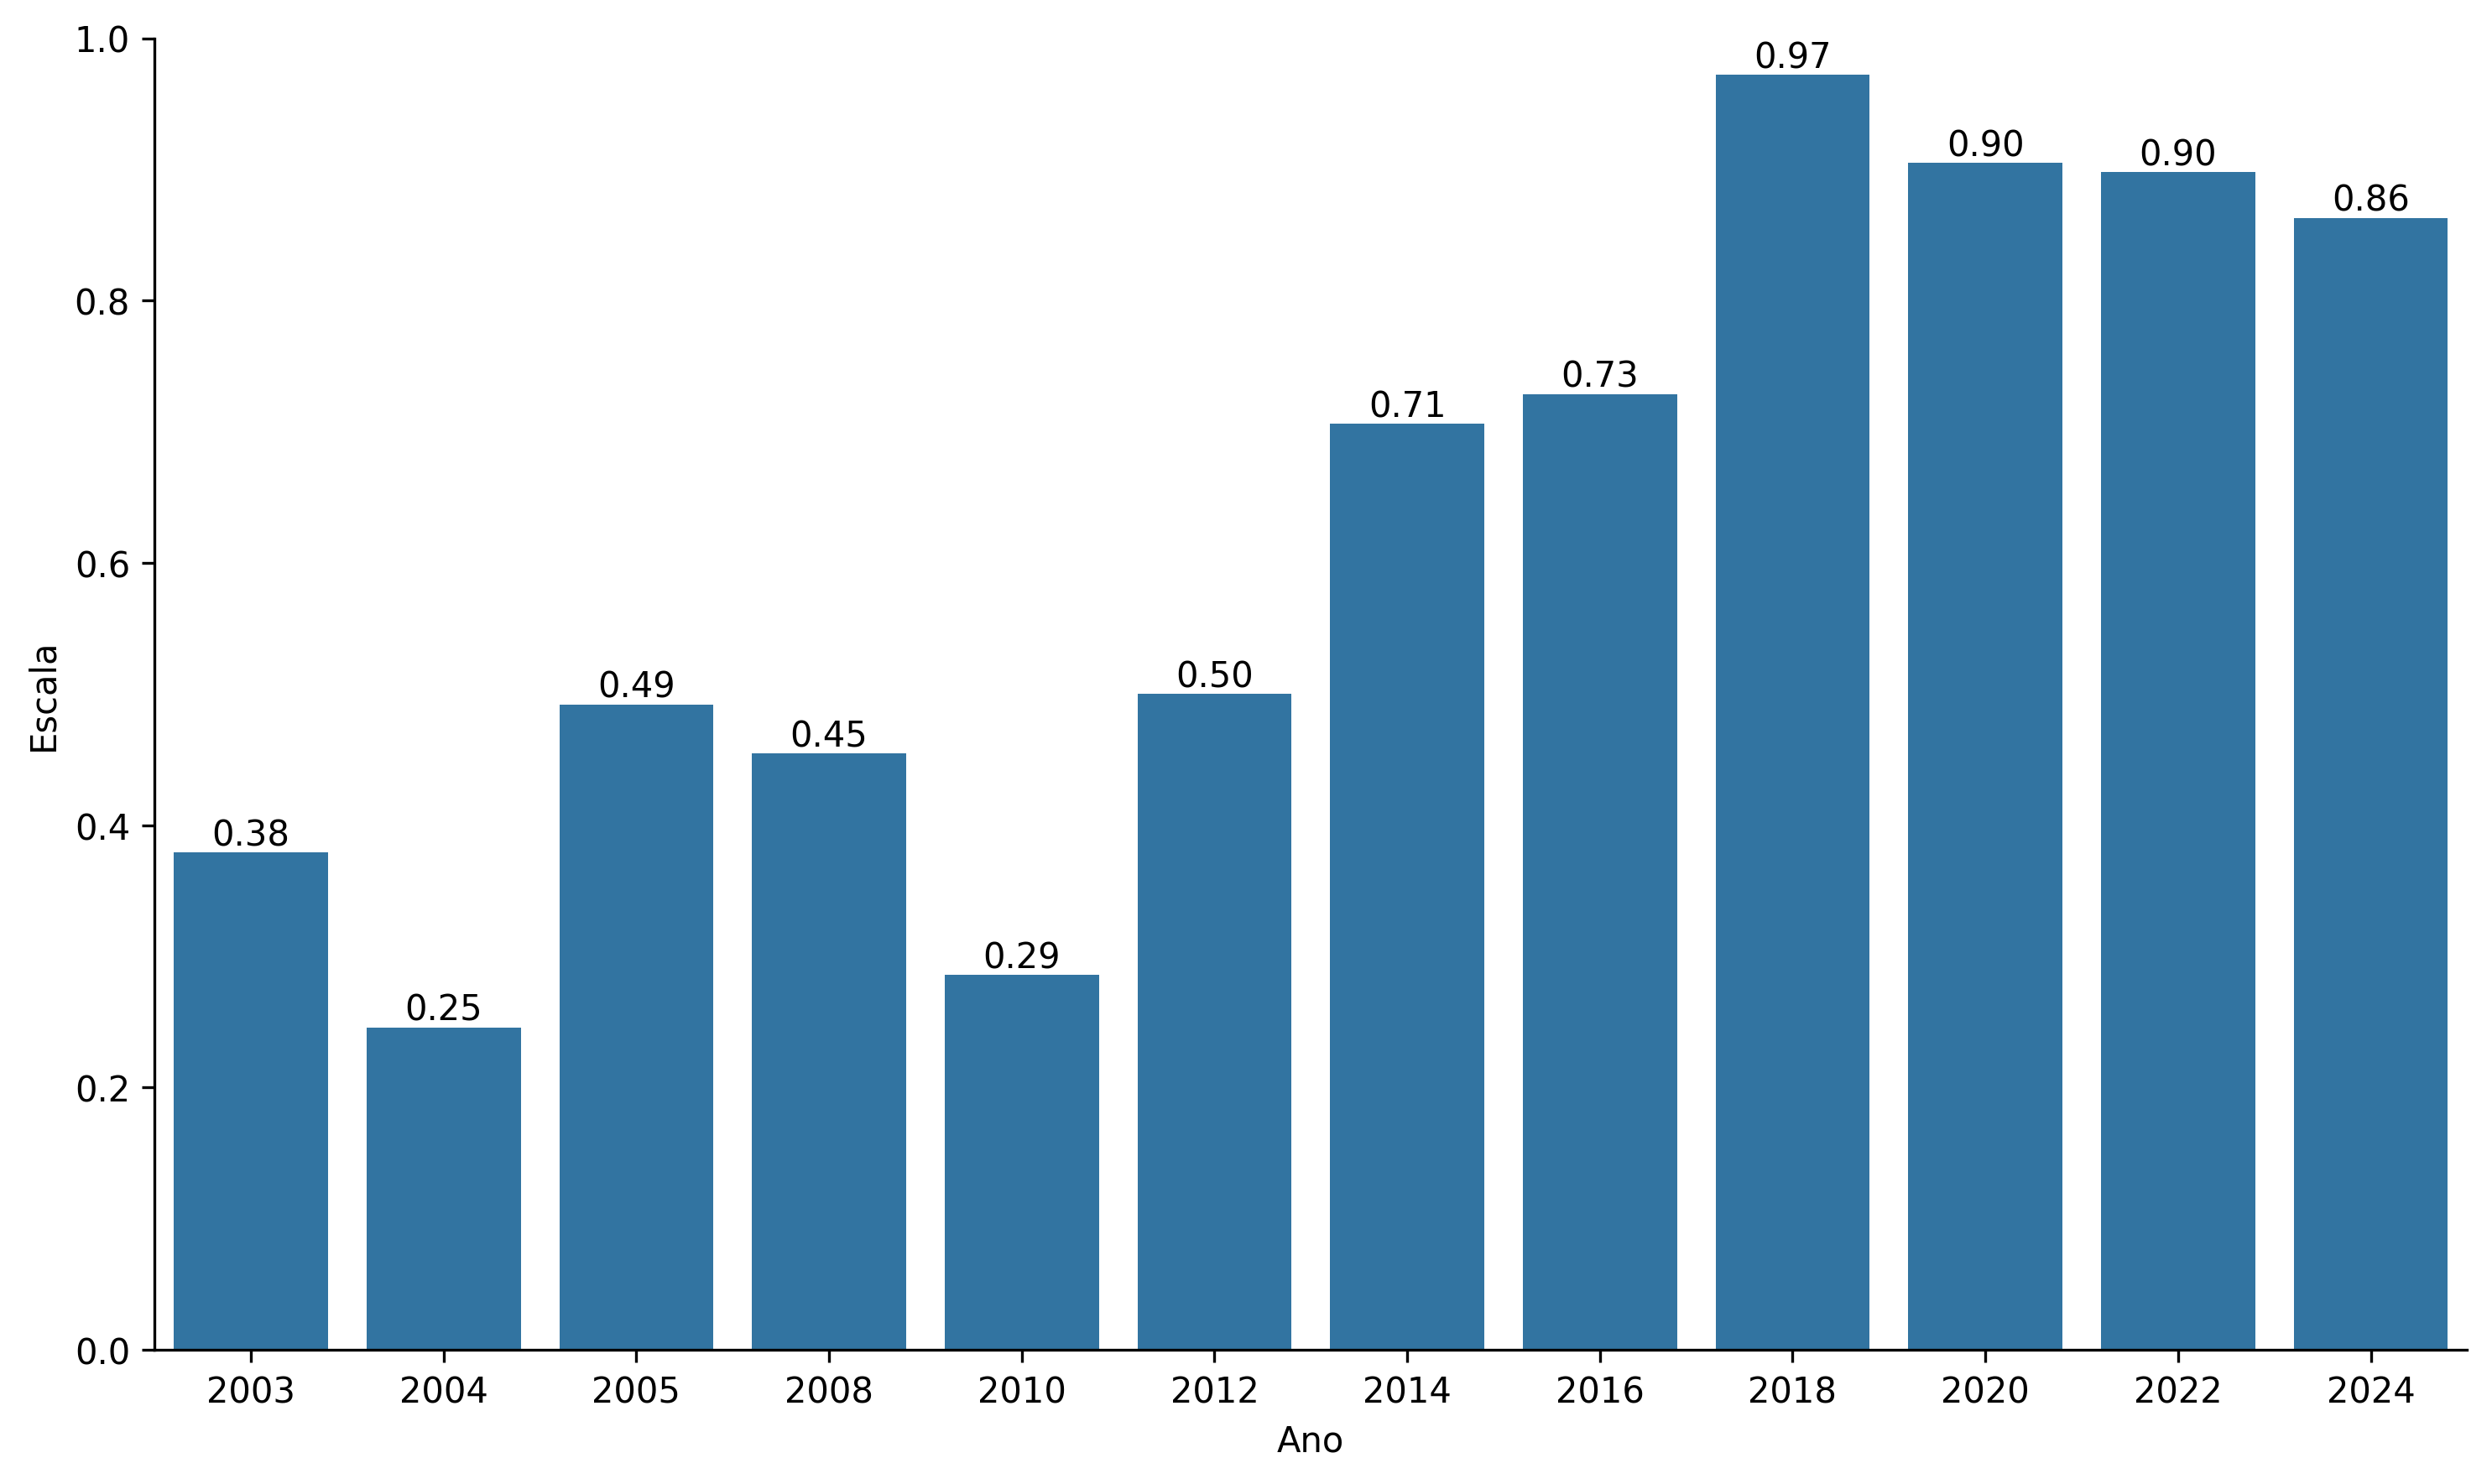
\includegraphics[width=1\linewidth]{figuras/egdi/egdi_brasil_epart.png}
	\label{fig:egdi_brasil_epart}
	\footnotesize{Fonte: baseado em \cite{ONU_edgi_mapa}.}
\end{figure}

\paragraph{Online Service Index}

\begin{figure}[H]
	\centering
	\caption{EGDI do Brasil: Online Service Index}
	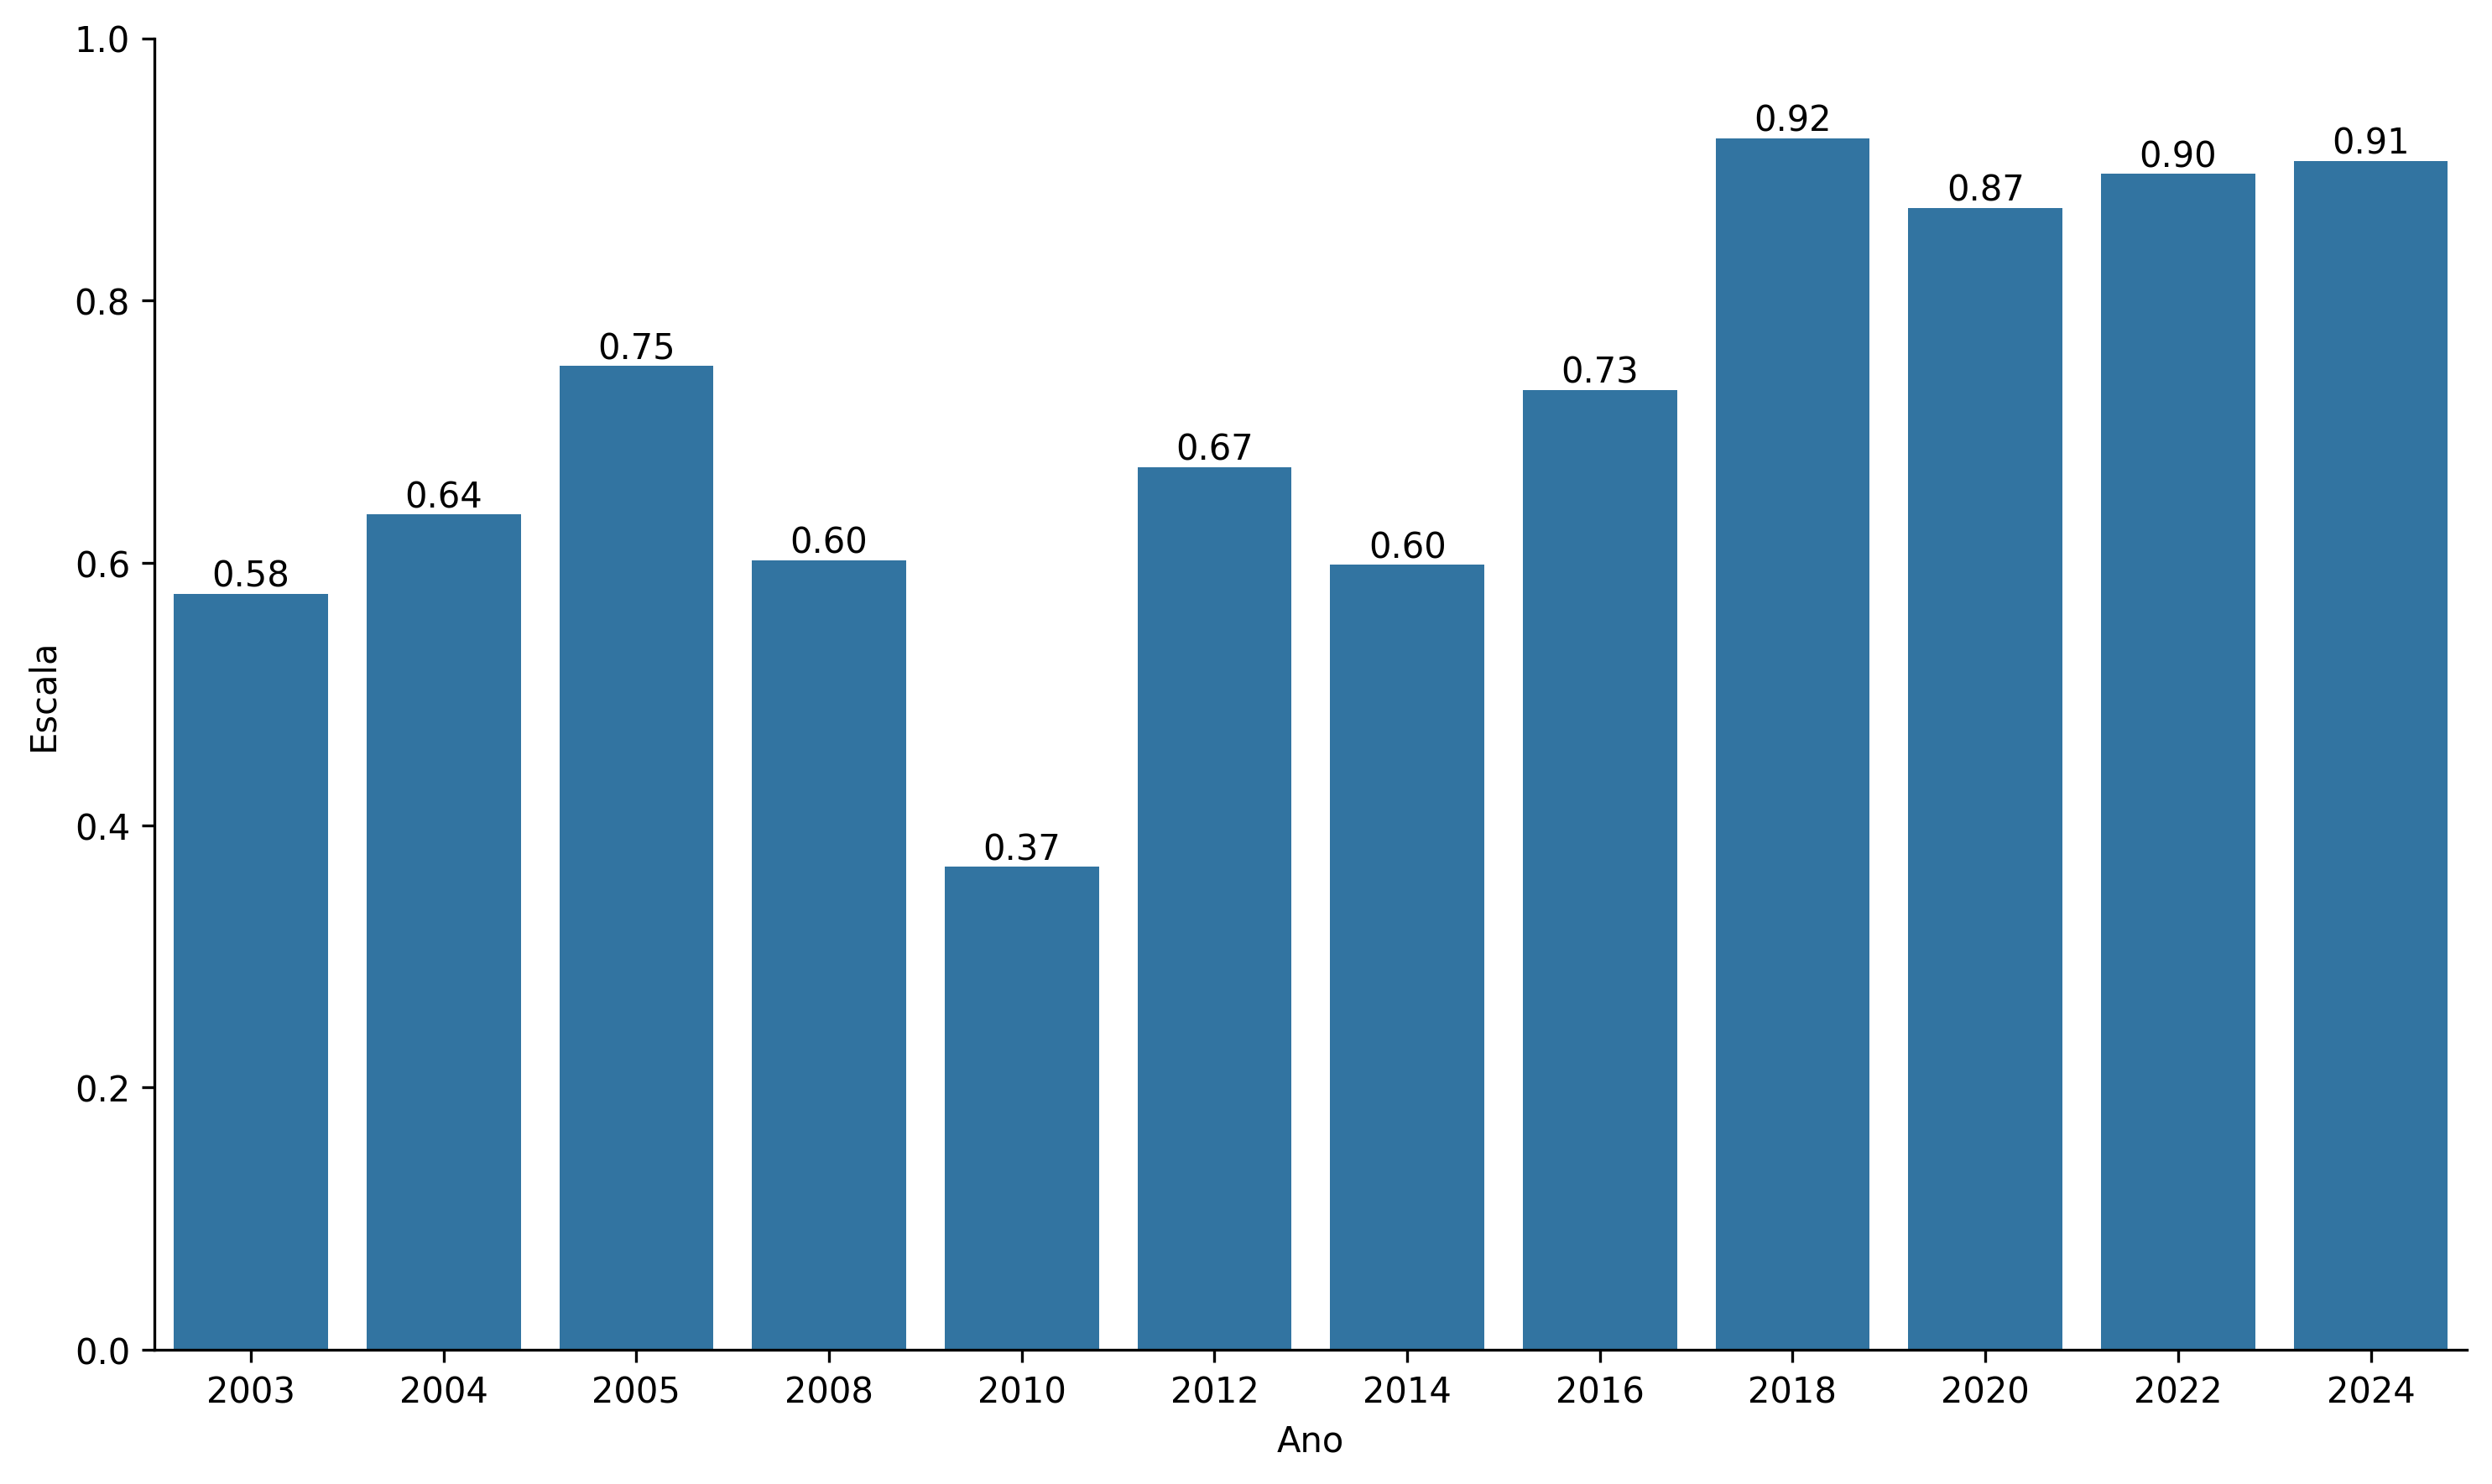
\includegraphics[width=1\linewidth]{figuras/egdi/egdi_brasil_osi.png}
	\label{fig:egdi_brasil_osi}
	\footnotesize{Fonte: baseado em \cite{ONU_edgi_mapa}.}
\end{figure}

\paragraph{Human Capital Indexx}

\begin{figure}[H]
	\centering
	\caption{EGDI do Brasil: Human Capital Index}
	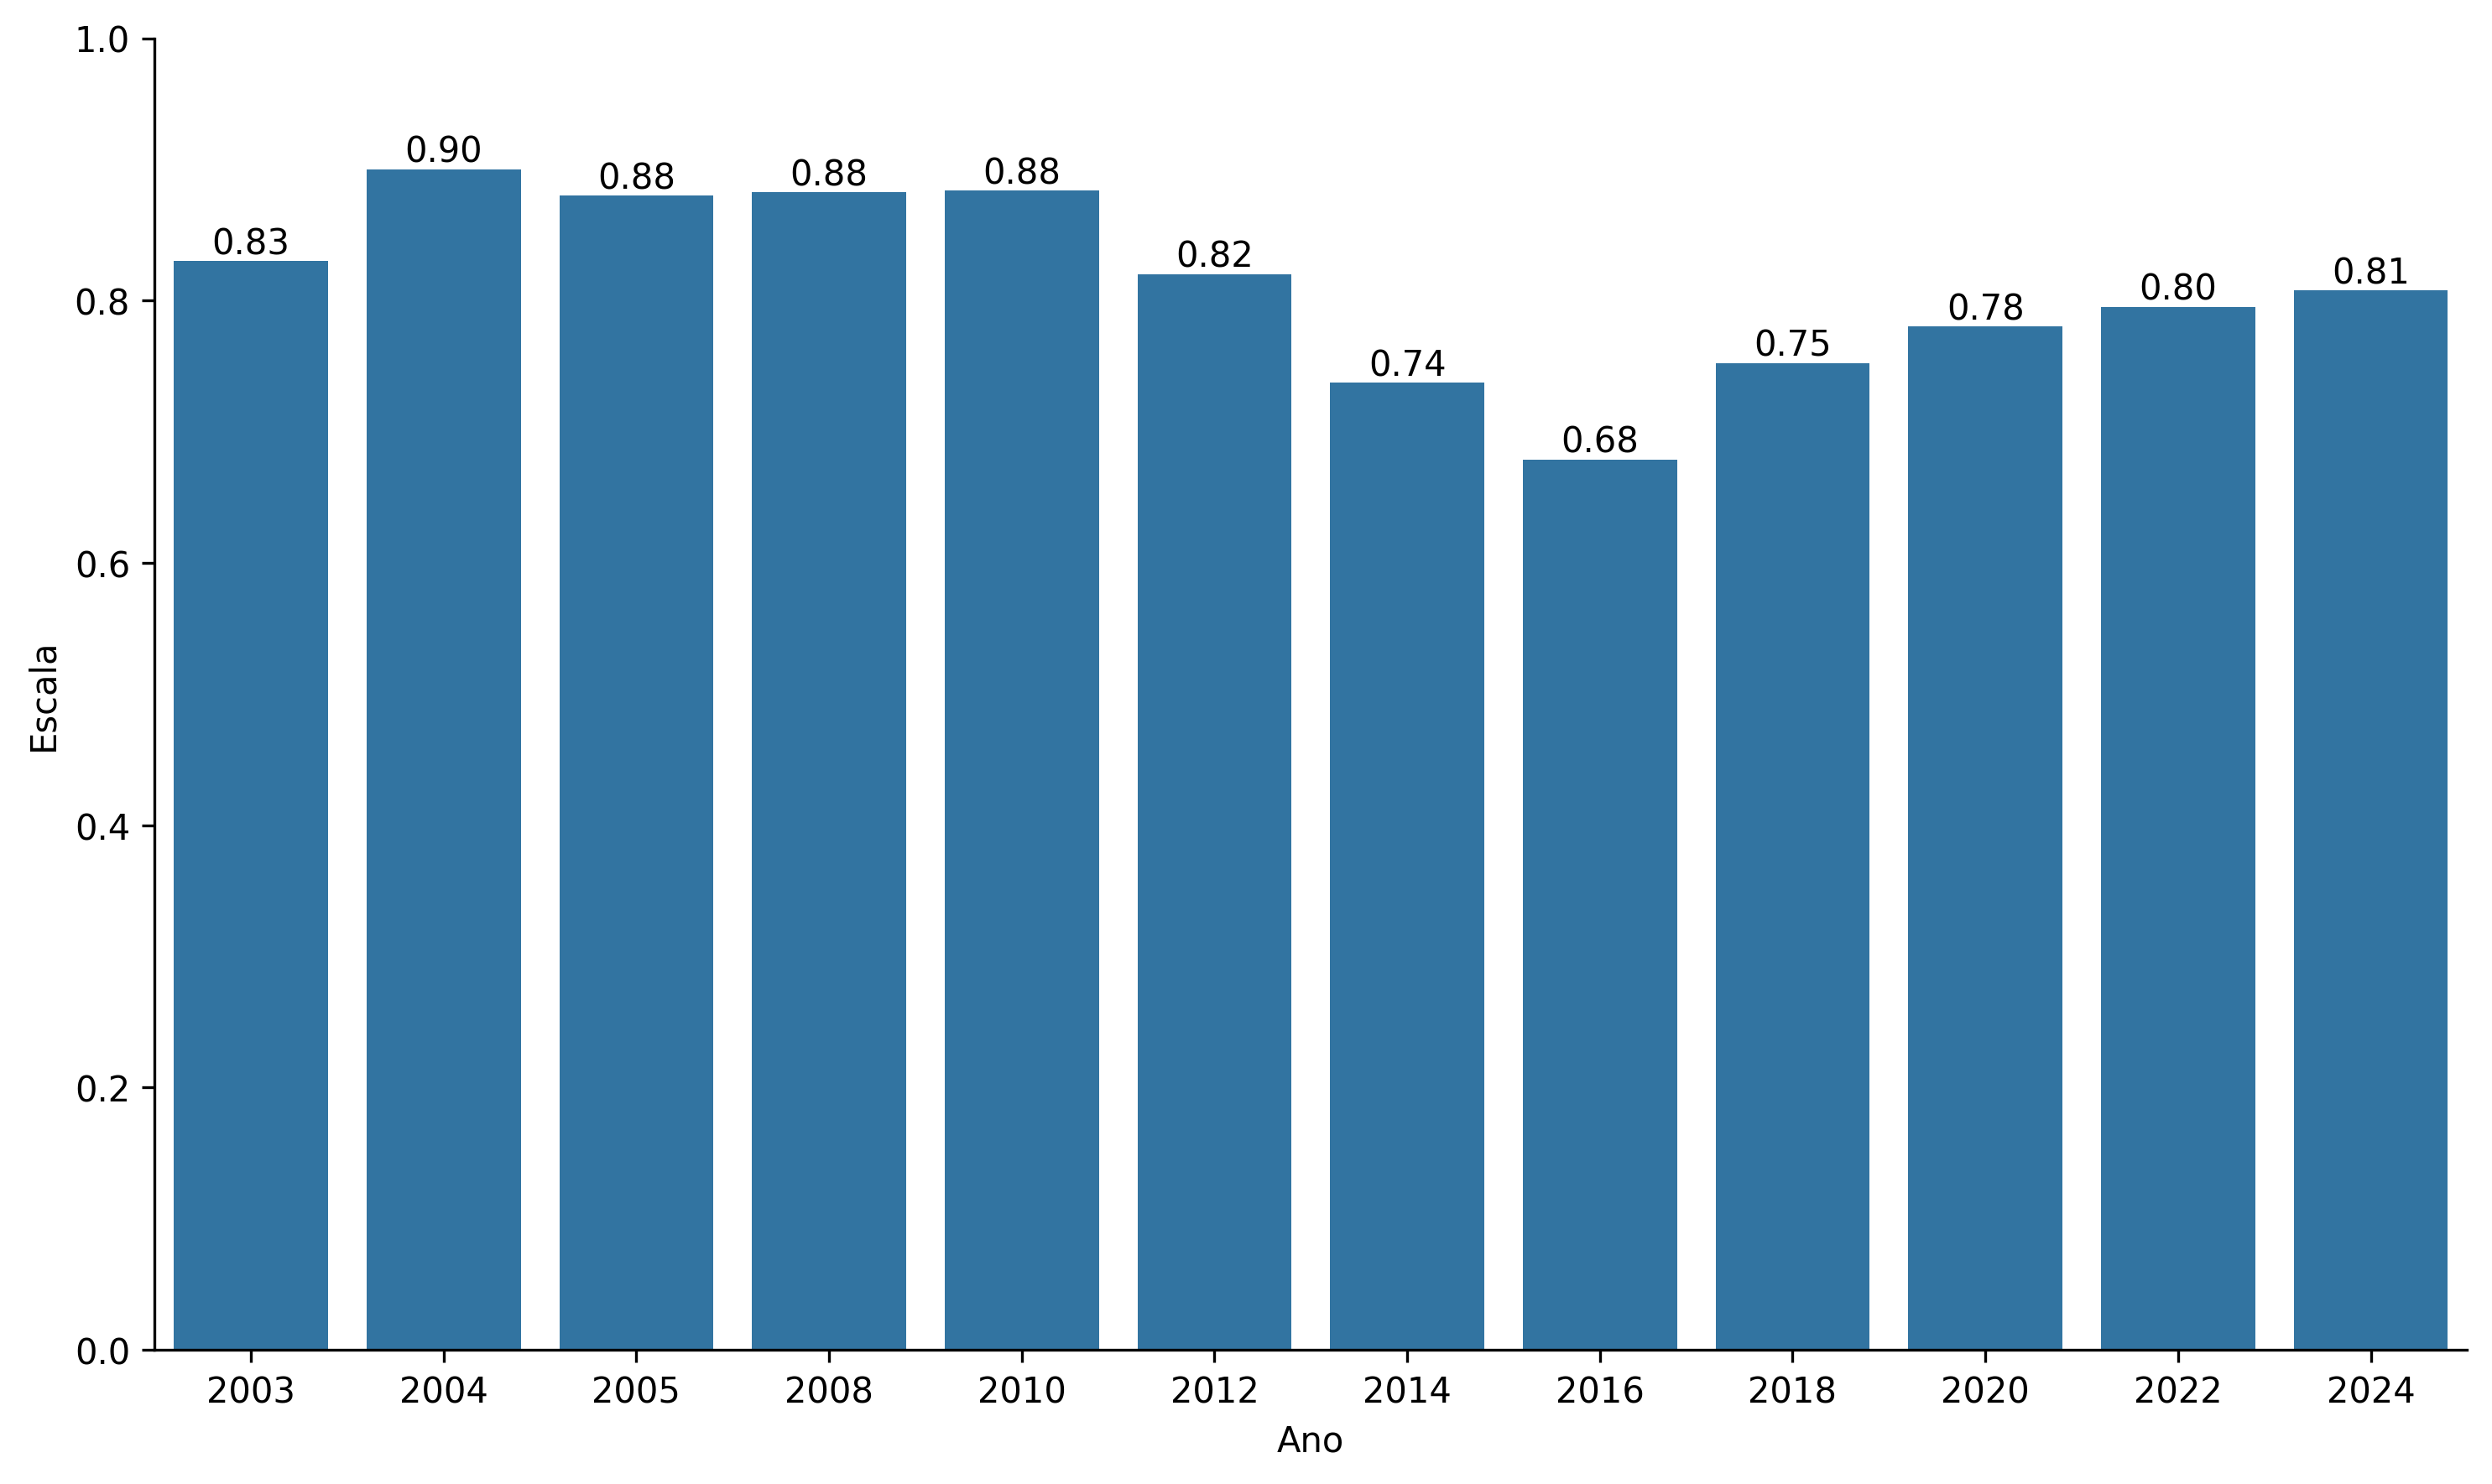
\includegraphics[width=1\linewidth]{figuras/egdi/egdi_brasil_hci.png}
	\label{fig:egdi_brasil_hci}
	\footnotesize{Fonte: baseado em \cite{ONU_edgi_mapa}.}
\end{figure}

\paragraph{Telecommunication Infrastructure Index}

\begin{figure}[H]
	\centering
	\caption{EGDI do Brasil: Telecommunication Infrastructure Index}
	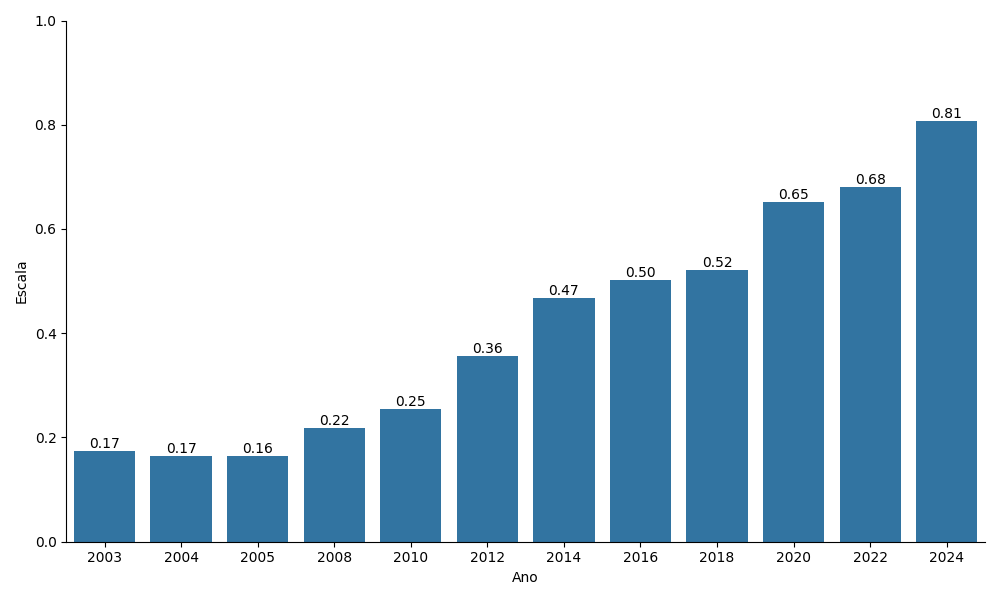
\includegraphics[width=1\linewidth]{figuras/egdi/egdi_brasil_tsi.png}
	\label{fig:egdi_brasil_tsi}
	\footnotesize{Fonte: baseado em \cite{ONU_edgi_mapa}.}
\end{figure}

\subsubsection{Coeficiente de correlação de Spearman: EGDI, índice de democracia eleitoral, PIB \textit{per capital} e uso de internet}

Ao analisar os dados do \href{https://publicadministration.un.org/egovkb/en-us/About/Overview/-E-Government-Development-Index}{EGDI}, foi notado que tanto democracias consolidadas, quanto autocracias tem um EGDI alto. O critério para entender quais países são democráticos ou autocráticos foram as figuras presentes no Apêndice \ref{demo_auto_mundo}. 

Nota-se que em qualquer figura o Brasil é considerado uma democracia (eleitoral, completa ou liberal), estão na minoria numérica de países democráticas (88), conforme exposto por \cite{nord2025democracy}, contra 91 autocracias.

Outro fator chamou atenção: há EGDI alto em países tanto autocráticos, quanto democráticos que têm PIB \textit{per capita} alto, conforme comparação dos \href{https://data.worldbank.org/indicator/NY.GDP.PCAP.PP.KD}{com o PIB \textit{per capita} dos países}. 

Em razão dos parágrafos anteriores, um questionamento surgiu: qual é relação entre EDGI e índice de democracia eleitoral do \href{https://www.v-dem.net/}{V-Dem}, o PIB \textit{per capita} e uso de internet tanto nos países do mundo, quanto no Brasil. Para responder a pergunta, foi usado o coeficiente de correlação de Spearman. O resultado foi dividido nas figuras \ref{fig:correlacao3}, \ref{fig:correlacao4}, \ref{fig:correlacao8} e \ref{fig:correlacao6}.

\begin{figure}[H]
    \centering
    \caption{Coeficiente de correlação de Spearman: índice de democracia eleitoral e o EGDI dos 193 países}
    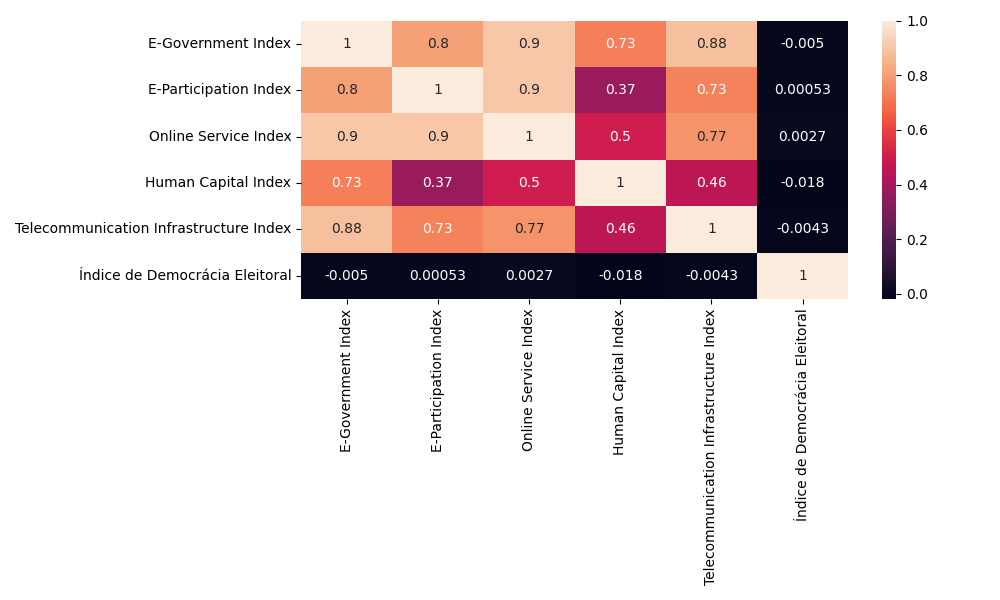
\includegraphics[width=1\linewidth]{figuras/egdi/correlacao3.png}
    \label{fig:correlacao3}
    \footnotesize{Fonte: baseado em \cite{ONU_edgi_mapa} e \cite{electoral_democracy_index}.}
\end{figure}

A \ref{fig:correlacao3} demonstra que não correlação entre o índice de democracia eleitoral e o EGDI dos 193 países. Ou seja, uma democracia ou autocracia pode ter um EGDI alto devido a outras variáveis, mas democracia não é uma delas.

\begin{figure}[H]
    \centering
    \caption{Coeficiente de correlação de Spearman: PIB \textit{per capita} PPC em USD e EGDI dos 193 países}
    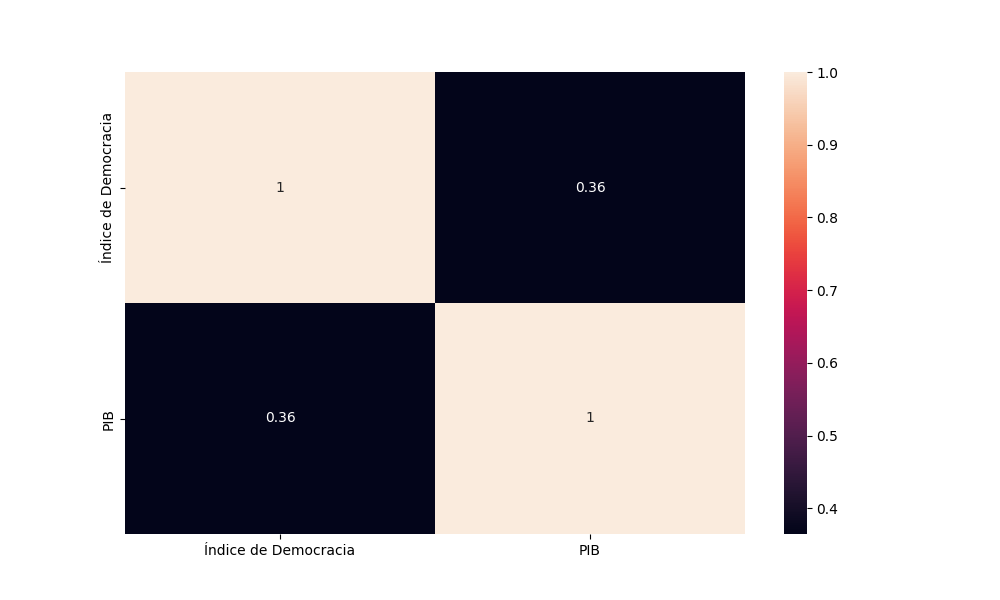
\includegraphics[width=1\linewidth]{figuras/egdi/correlacao4.png}
    \label{fig:correlacao4}
    \footnotesize{Fonte: baseado em \cite{ONU_edgi_mapa} e \cite{WB_pib_per_capita_países}.}
\end{figure}

A \ref{fig:correlacao4} demonstra que não correlação entre o PIB \textit{per capita} PPC e o EGDI dos 193 países. Ou seja, uma democracia ou autocracia pode ter um EGDI alto devido a outras variáveis, mas o PIB \textit{per capita} PPC de qualquer valor não tem interferência.

A análise global mostrou resultados interessantes. No entanto, diminui-se o escopo de análise para o Brasil.

\begin{figure}[H]
    \centering
    \caption{Coeficiente de correlação de Spearman: índice de democracia eleitoral e o EGDI do Brasil}
    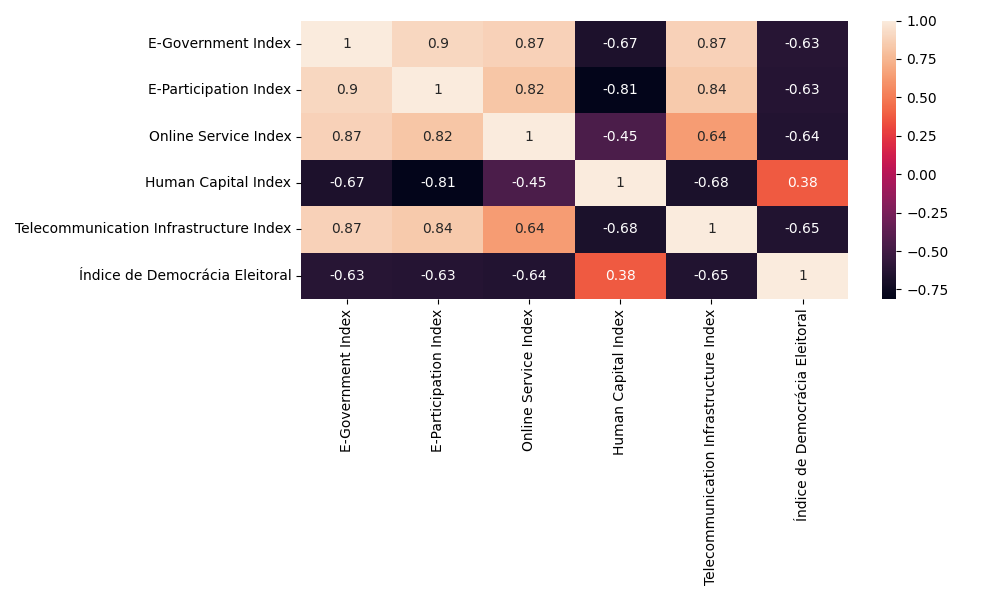
\includegraphics[width=1\linewidth]{figuras/egdi/correlacao8.png}
    \label{fig:correlacao8}
    \footnotesize{Fonte: baseado em \cite{ONU_edgi_mapa} e \cite{electoral_democracy_index}.}
\end{figure}

Apenas o Human Capital Index teve uma correlação positiva de 0.38 com o índice de democracia eleitoral do Brasil.

\begin{figure}[H]
    \centering
    \caption{Coeficiente de correlação de Spearman: PIB \textit{per capita} PPC em USD e EGDI do Brasil}
    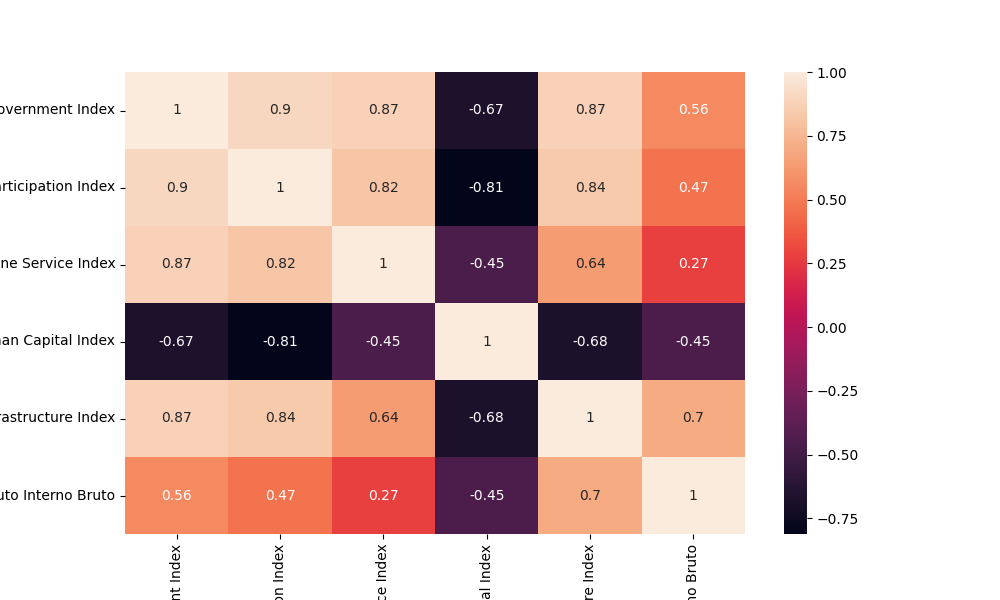
\includegraphics[width=1\linewidth]{figuras/egdi/correlacao6.png}
    \label{fig:correlacao6}
    \footnotesize{Fonte: baseado em \cite{ONU_edgi_mapa} e \cite{WB_pib_per_capita_países}.}
\end{figure}


\subsubsection{Indicadores de TIC de governo eletrônico}

A ONU tem \href{https://publicadministration.un.org/egovkb/en-us/Data/ICT-in-government}{indicadores de TIC de governo eletrônico} como algo complementar ao EGDI. Os indicadores são, conforme \cite{ONU_ICT_in_government_indicators}:

\begin{itemize}
    \item Existência de estratégia nacional de governo eletrônico ou equivalente;
    \item Existência de identidade digital para acessar ou outra forma de autenticação requirida para poder acessar serviços online;
    \item Existência de um portal de compras governamentais.
\end{itemize}

Os resultados globais dos indicadores estão presentes nas figuras \ref{fig:national_government_strategy}, \ref{fig:national_identity} e \ref{fig:procurement_portal}.

\begin{figure}[H]
	\centering
	\caption{Indicador: Existência de estratégia nacional de governo eletrônico ou equivalente}
	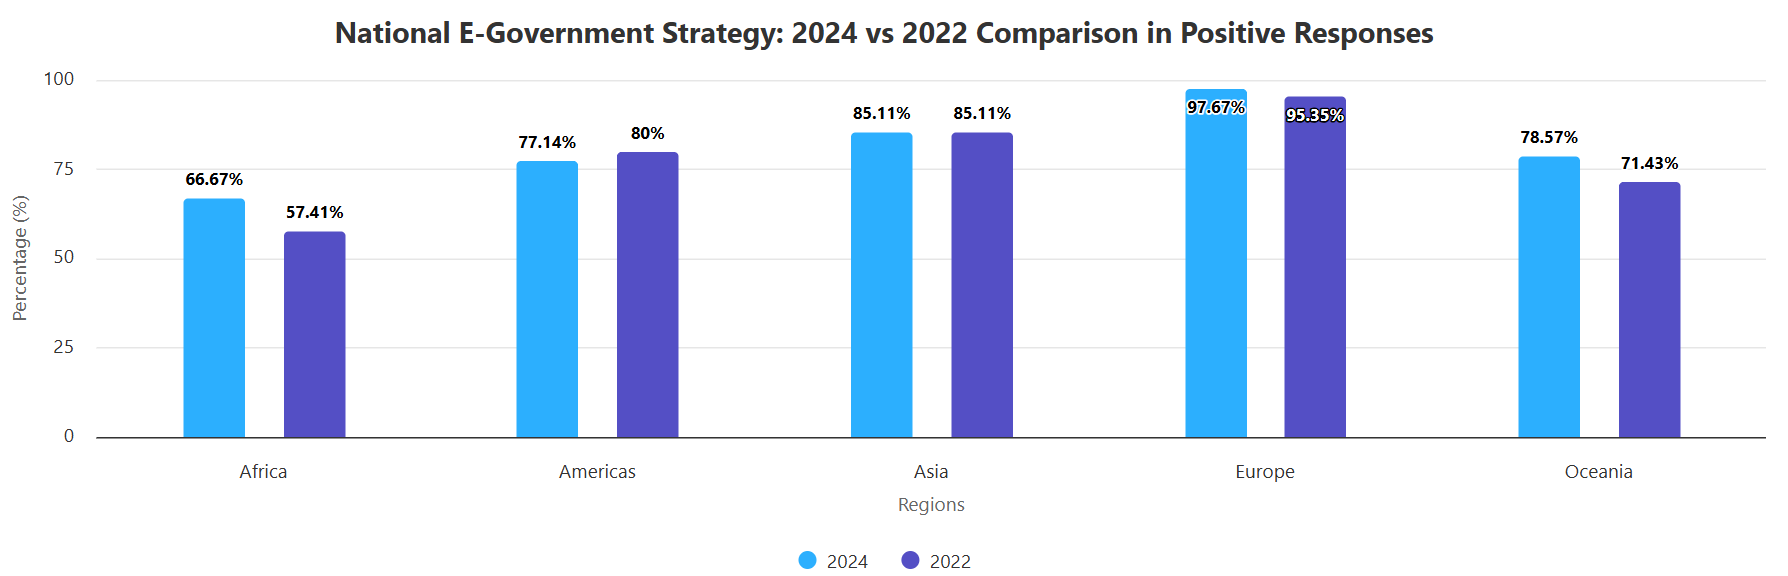
\includegraphics[width=1\linewidth]{figuras/ict_in_government/national_government_strategy}
	\label{fig:national_government_strategy}
	\footnotesize{Fonte: \cite{ONU_ICT_in_government_indicators}}
\end{figure}

\begin{figure}[H]
	\centering
	\caption{Indicador: Existência de identidade digital para acessar ou outra forma de autenticação requirida para poder acessar serviços online}
	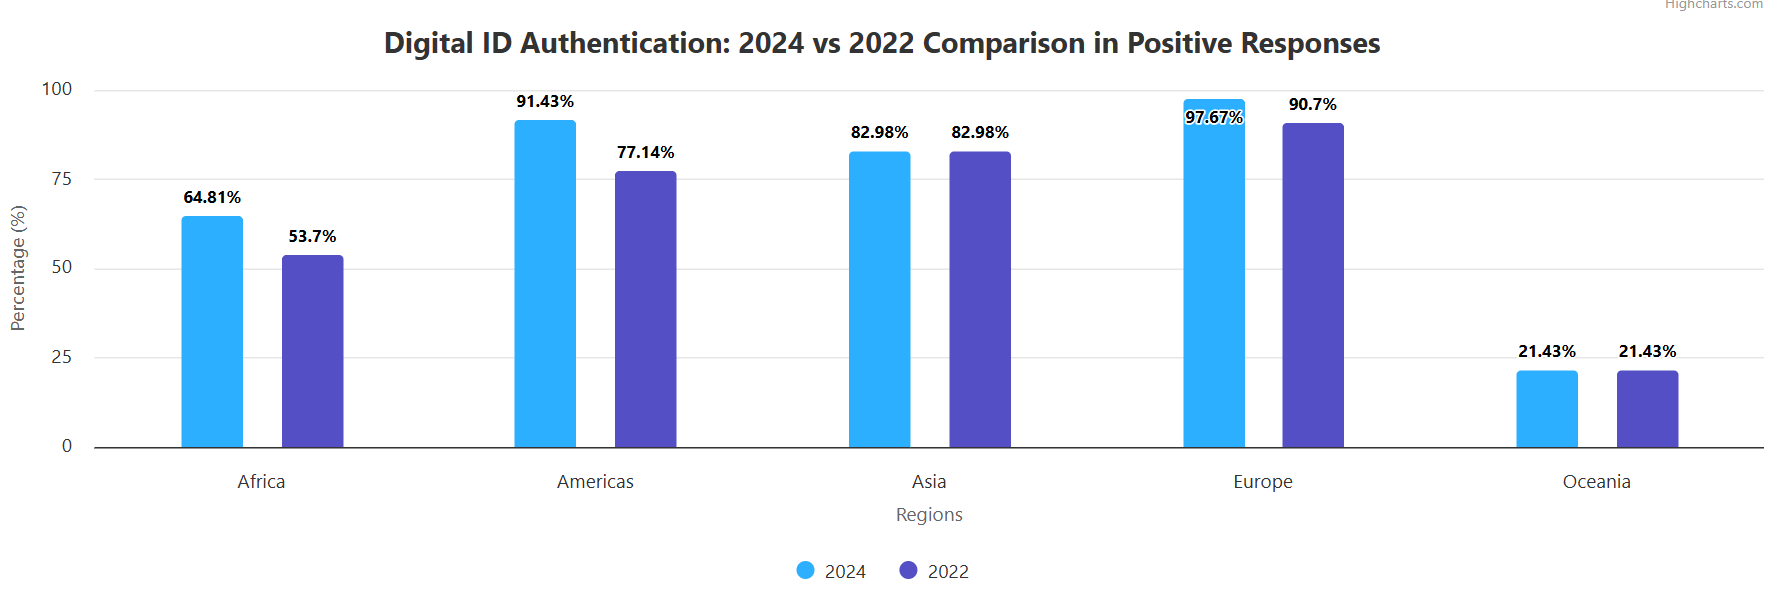
\includegraphics[width=1\linewidth]{figuras/ict_in_government/digital_identity}
	\label{fig:national_identity}
	\footnotesize{Fonte: \cite{ONU_ICT_in_government_indicators}}
\end{figure}

\begin{figure}[H]
	\centering
	\caption{Indicador: Existência de um portal de compras governamentais}
	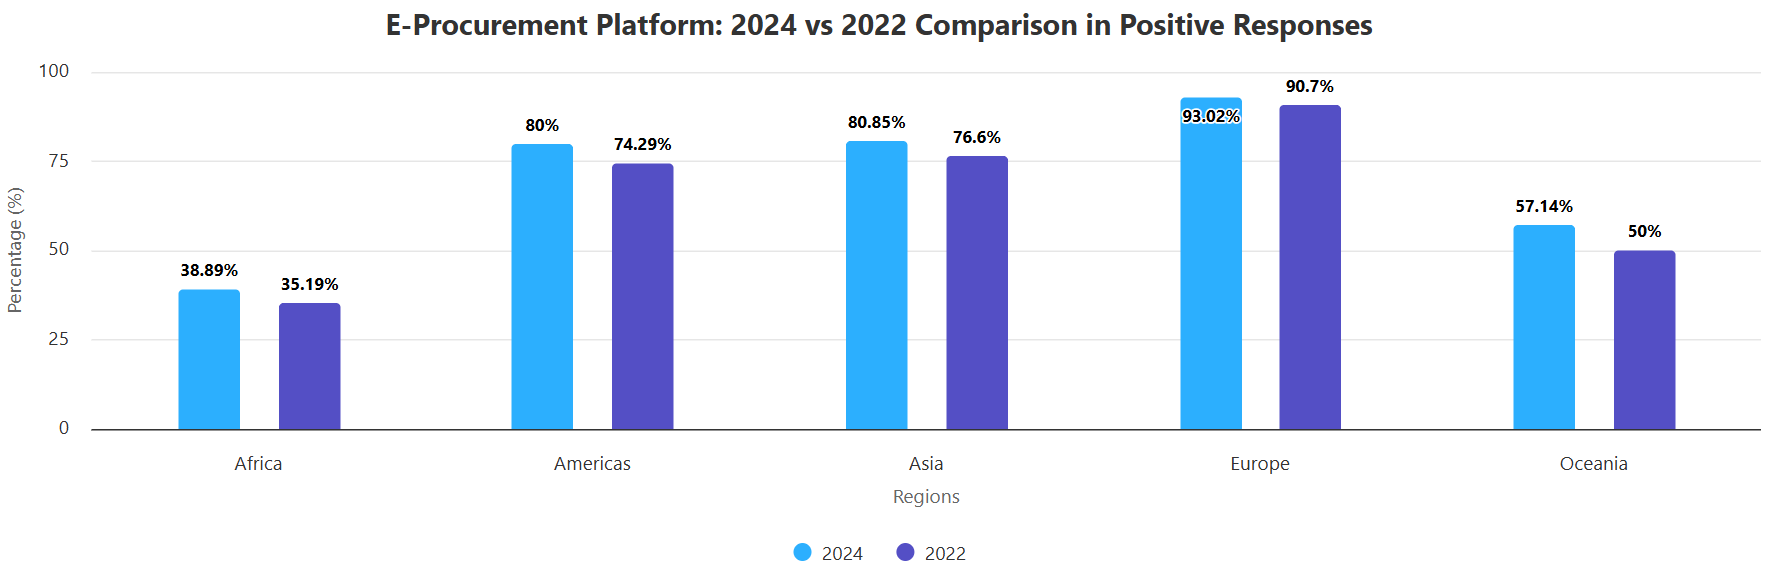
\includegraphics[width=1\linewidth]{figuras/ict_in_government/procurement_portal}
	\label{fig:procurement_portal}
	\footnotesize{Fonte: \cite{ONU_ICT_in_government_indicators}}
\end{figure}

Das três figuras, a Europa foi o continente cujos mais respondem que têm seguem os indicadores, superando os 90\%. A Oceania foi o continente que menos implementou políticas de identidade digital para acesso a serviços online. África e Oceania tiveram um desempenho ruim na implementação de portais de compra governamentais. O continente americano apresentou bom desempenho nos três indicadores.

Como consequência da análise dos resultados presentes nas figuras \ref{fig:national_government_strategy}, \ref{fig:national_identity} e \ref{fig:procurement_portal}, buscou-se entender a seguinte situação registrada nos 2022 e 2024, anos em que os indicadores foram medidos: qual é a porcentagem de países que responderam nenhuma, uma, duas ou todas as perguntas. Elas usam sim ou não para confirmar a aplicação dos indicadores no país.

A resposta ao questionamento está presente na figura \ref{fig:indicators_answer}.

\begin{figure}[H]
	\centering
	\caption{Resposta positiva aos indicadores de TIC de governo eletrônico}
	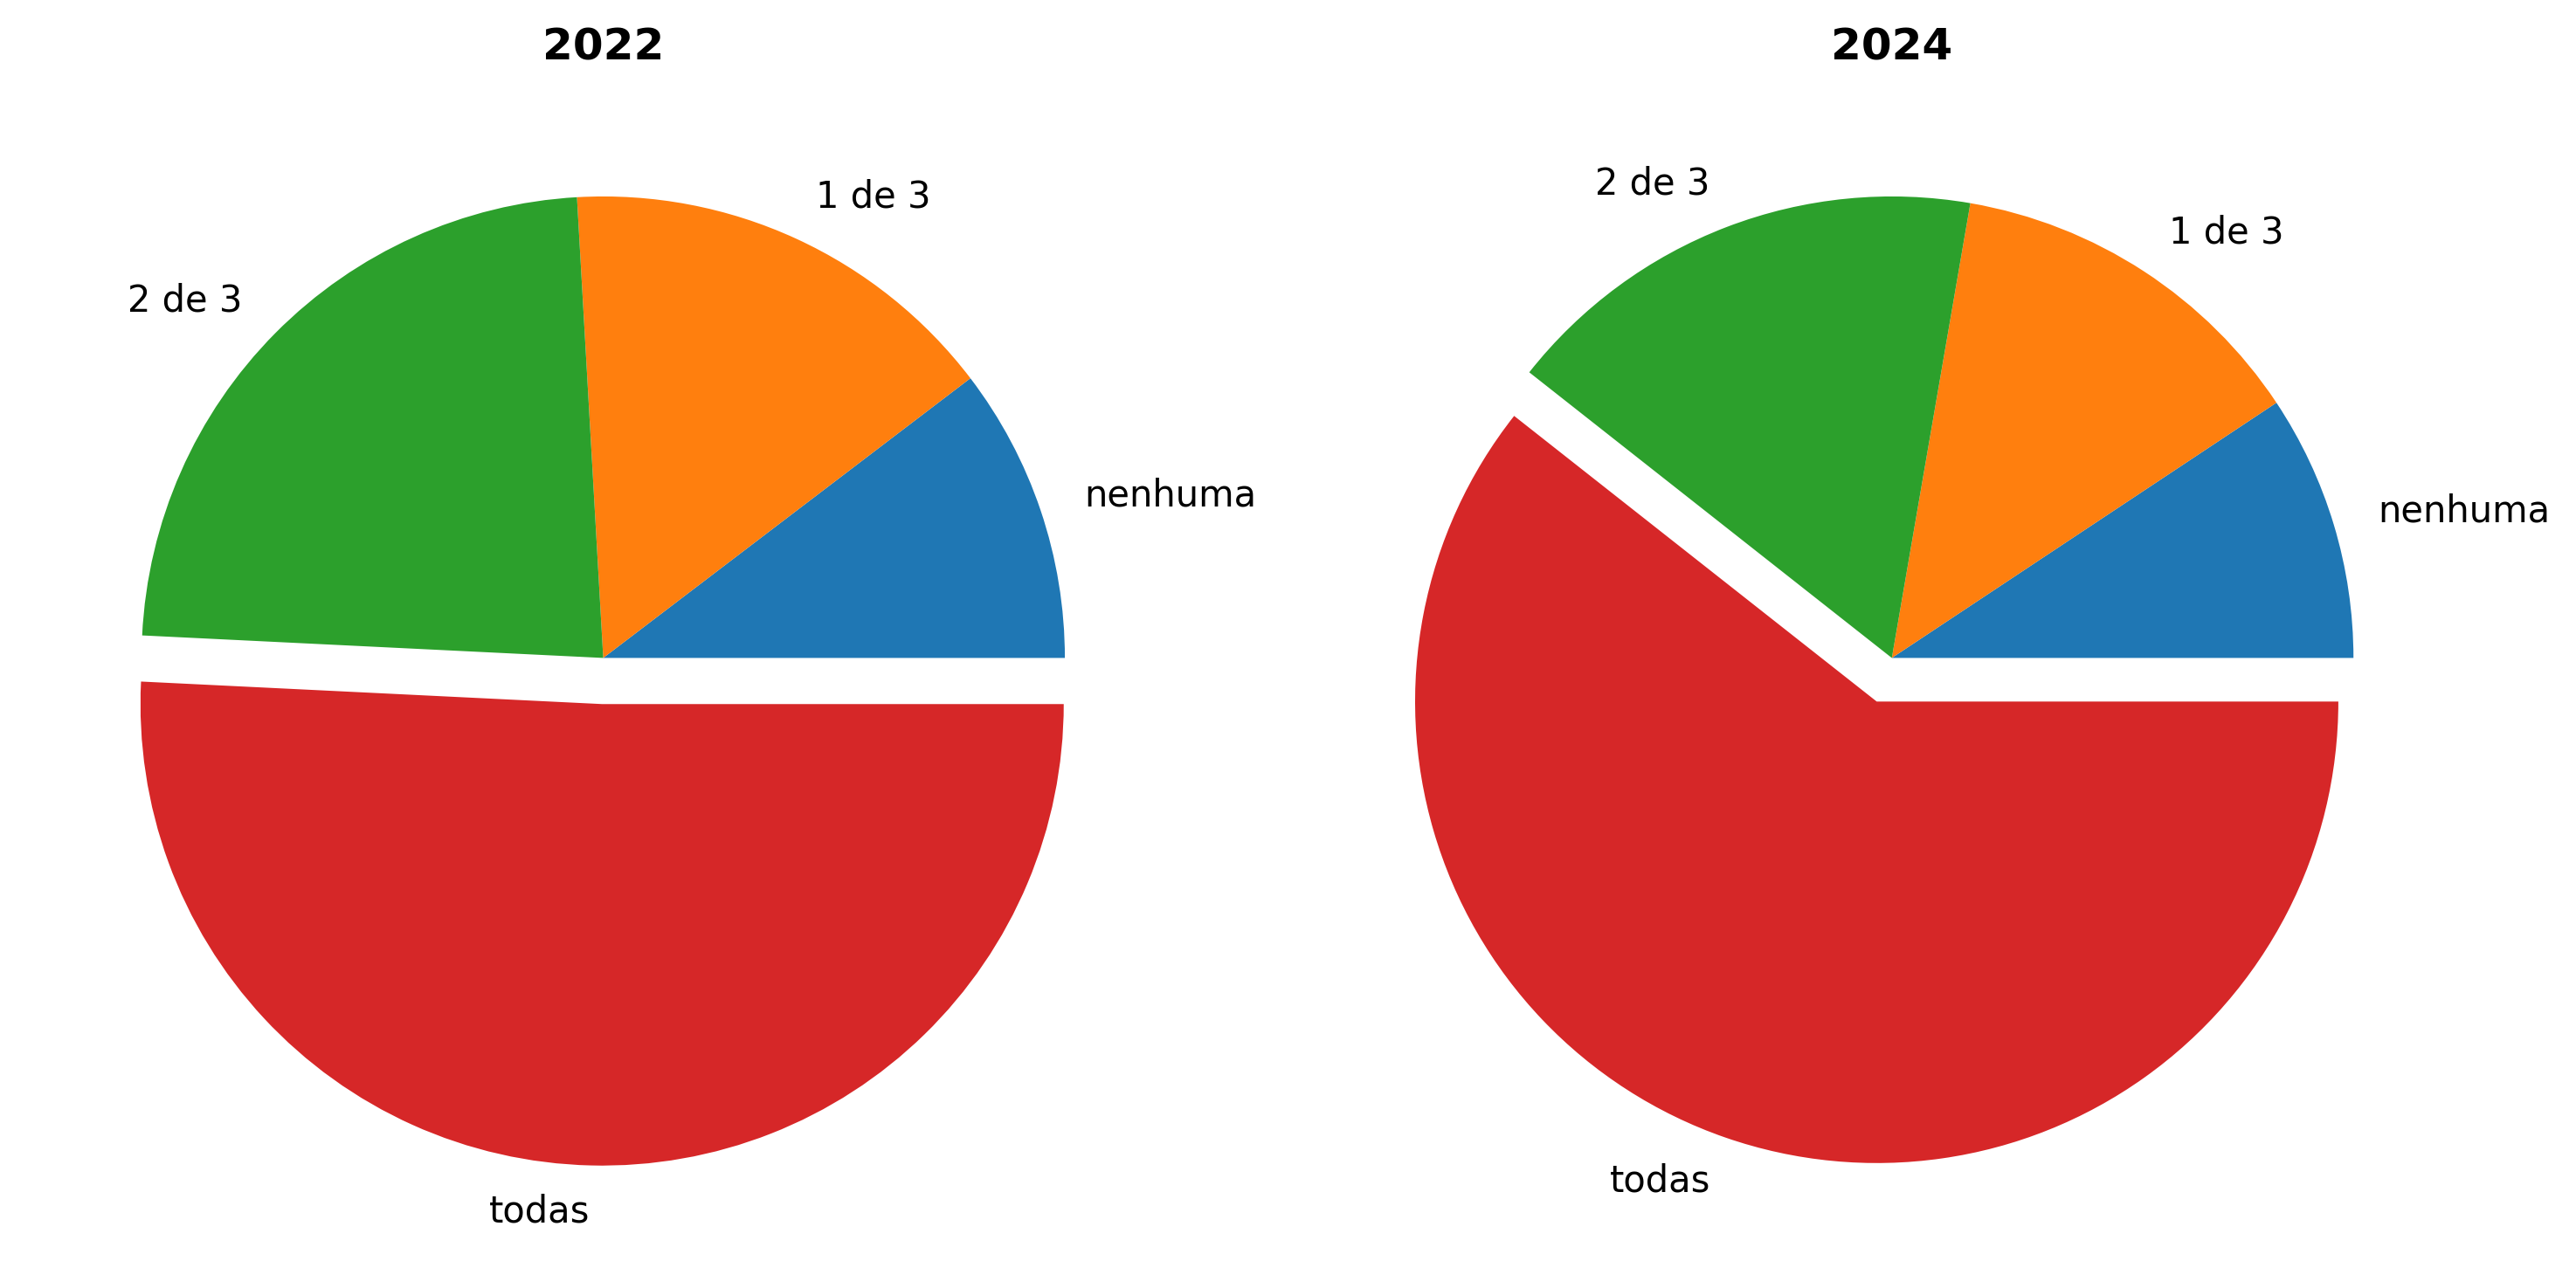
\includegraphics[width=1\linewidth]{figuras/ict_in_government/indicators_answer}
	\label{fig:indicators_answer}
	\footnotesize{Fonte: \cite{ONU_ICT_in_government_indicators}}
\end{figure}

Em 2022, metade dos países respondeu positivamente as três perguntas; em 2024, mais da metade. O Brasil faz parte desse grupo, tal como a Rússia e China. A mudança é creditada a redução do número de países que responderam positivamente 2 de 3 perguntas e passaram a responder as três positivamente. 

Além, disso a quantidade de países que responderam positivamente 1 de 3 perguntas e nenhuma se igualou em 2024, sendo os países que responderam 1 de 3 perguntas era maior do que os que responderam nenhuma.

Tal detalhe se alinha à não correlação entre o EGDI e o índice de democracia eleitoral. Porém, buscou-se entender se há correlação entre os indicadores de TIC de governo eletrônico e o PIB \textit{per capita} PPC.